\documentclass[12pt,UTF8]{ctexart}
\usepackage{ctex,amsmath,amssymb,geometry,fancyhdr,bm,amsfonts,mathtools,extarrows,graphicx,url,enumerate,color,float,multicol,subfig} 
\allowdisplaybreaks[4]
% 加入中文支持
\newcommand\Set[2]{\left\{#1\ \middle\vert\ #2 \right\}}
\newcommand\Lim[0]{\lim\limits_{n\rightarrow\infty}}
\newcommand\Ser[1]{\sum_{n=#1}^\infty}
\newcommand{\SER}[2]{\sum_{#1=#2}^\infty}
\geometry{a4paper,scale=0.80}
\pagestyle{fancy}
\rhead{习题8.4\&8.5\&8.6}
\lhead{基础习题课讲义}
\chead{微积分B(1)}
\begin{document}
\setcounter{section}{12}
\section{函数级数}
\noindent
\subsection{知识结构}
\noindent第8章级数
	\begin{enumerate}
		\item[8.4]函数级数
			\begin{enumerate}
				\item[8.4.1]函数级数及其收敛域
				\item[8.4.2]函数级数的一致收敛性
				\item[8.4.3]一致收敛级数的分析性质
			\end{enumerate}
		\item[8.5]幂级数
			\begin{enumerate}
				\item[8.5.1]幂级数的收敛半径与收敛域
				\item[8.5.2]幂级数的分析性质
				\item[8.5.3]函数的幂级数展开
				\item[8.5.4]幂级数求和
			\end{enumerate}
		\item[8.6]傅里叶级数
			\begin{enumerate}
				\item[8.6.1]周期函数的傅里叶级数
				\item[8.6.2]正弦级数与余弦级数
				\item[8.6.3]傅里叶级数的复数形式
				\item[8.6.4]傅里叶级数的平均收敛
			\end{enumerate}
	\end{enumerate}
\subsection{习题8.4解答}
\begin{enumerate}
\item求下列函数项级数的收敛域,并指出使级数绝对收敛、条件收敛的$x$的范围:
\newline
\begin{tabular}{ll}
(1)$\Ser{1}n\mathrm e^{-nx}$;&(2)$\Ser{1}(\frac{\lg x}2)^n$;\\
(3)$\Ser{1}x^n\ln(1+\frac1{2^n})$;&(4)$\Ser{1}\frac1{n+x^n}$;\\
(5)$\Ser{6}\frac{(-1)^n}{(n^2-4n-5)^x}$;&(6)$\Ser{1}\frac{x^n}{1+x^{2n}}$;\\
(7)$\Ser{1}\frac{(-1)^n}{n+x^2}$;&(8)$\Ser{1}\frac{n5^{2n}}{6^n}x^n(1-x)^n$.
\end{tabular}

解:(1)$\because\Lim\frac{u_{n+1}}{u_n}=\Lim\frac{(n+1)\mathrm e^{-(n+1)x}}{n\mathrm e^{-nx}}=\frac1{\mathrm e^x}$

$\therefore$当$\frac1{\mathrm e^x}<1$即$x>0$时,该正项级数绝对收敛;当$\frac1{\mathrm e^x}>1$即$x<0$时,级数发散;当$x=0$时,级数为$\Ser{1}n$发散,故级数的收敛域为$(0,+\infty)$.

(2)$\because\Lim\sqrt[n]{|(\frac{\lg x}2)^n|}=|\frac{\lg x}2|$

$\therefore$当$|\frac{\lg x}2|<1$即$\frac1{100}<x<100$时,级数绝对收敛;

当$|\frac{\lg x}2|>1$即$0<x<\frac1{100}$或$x>100$时,$\Lim(\frac{\lg x}2)^n=+\infty$级数发散;

当$|\frac{\lg x}2|=1$即$x=\frac1{100}$或$x=100$时,$\Lim(\frac{\lg x}2)^n=\Lim(\frac{\pm2}2)^n\neq0$级数发散.

故级数的收敛域为$(\frac1{100},100)$.

(3)$\because\Lim\frac{|u_{n+1}|}{|u_n|}=\Lim\frac{|x|^{n+1}\ln(1+\frac1{2^{n+1}})}{|x|^n\ln(1+\frac1{2^n})}=|x|\Lim\frac{\frac1{2^{n+1}}}{\frac1{2^n}}=\frac{|x|}2$

$\therefore$当$|x|<2$时级数绝对收敛

当$|x|>2$时$\Lim x^n\ln(1+\frac1{2^n})=\Lim x^n\frac1{2^n}=\Lim(\frac x2)^n=\infty$,级数发散;

当$|x|=2$时$\Lim x^n\ln(1+\frac1{2^n})=\Lim(\pm2)^n\frac1{2^n}\neq0$,级数发散.

故级数的收敛域为$(-2,2)$.

(4)当$|x|>1$时$\Lim n^2\cdot|\frac1{n+x^n}|=\Lim\frac{\frac{n^2}{|x|^n}}{\frac n{|x|^n}+(-1)^n}=0$,级数绝对收敛;

当$|x|<1$时$\Lim n\cdot\frac1{n+x^n}=1$,级数发散;

当$x=1$时级数$\Ser{1}\frac1{n+x^n}=\Ser{1}\frac1{n+1}$发散;

当$x=-1$时$\frac1{n+x^n}=\frac1{n+(-1)^n}\geq\frac1{n+1}$,级数发散.

故级数的收敛域为$(-\infty,-1)\cup(1,+\infty)$.

(5)$\because\Lim n^{2x}\cdot|\frac{(-1)^n}{(n^2-4n-5)^x}|=\Lim(\frac{n^2}{n^2-4n-5})^x=1$

$\therefore$当$2x>1$即$x>\frac12$时,级数绝对收敛;

当$0<2x\leq1$即$0<x\leq\frac12$时,由$\frac1{(n^2-4n-5)^x}$单调减少且$\Lim\frac1{(n^2-4n-5)^x}=0$知,级数条件收敛;

当$x=0$时,$\Ser{6}\frac{(-1)^n}{(n^2-4n-5)^x}=\Ser{6}(-1)^n$发散;

当$x<0$时,$\Lim\frac{(-1)^n}{(n^2-4n-5)^x}=\infty$,级数发散.

故级数的收敛域为$(0,+\infty)$.

(6)$\because\Lim\frac{|u_{n+1}|}{|u_n|}=\Lim\frac{|x|^{n+1}}{1+x^{2n+2}}\frac{1+x^{2n}}{|x|^n}=\Lim|x|\frac{1+x^{2n}}{1+x^{2n+2}}=\Lim|x|\frac{\frac1{x^{2n}}+1}{\frac1{x^{2n}}+x^2}=\begin{cases}
|x|<1,&|x|<1\\
1,&|x|=1\\
\frac1{|x|}<1,&|x|>1
\end{cases}$

$\therefore$当$|x|\neq1$时级数绝对收敛

当$|x|=1$时$\Lim\frac{x^n}{1+x^{2n}}=\Lim\frac{(\pm1)^n}{1+1}\neq0$,级数发散.

故级数的收敛域为$(-\infty,-1)\cup(-1,1)\cup(1,+\infty)$.

(7)由$|u_n|=\frac1{n+x^2}>\frac1{n+1+x^2}=|u_{n+1}|$且$\Lim\frac1{n+x^2}=0$知级数为莱布尼茨型交错级数,故收敛,

又由$\Lim n\cdot|\frac{(-1)^n}{n+x^2}|=\Lim\frac n{n+x^2}=1$可知级数条件收敛.

级数的收敛域为$(-\infty,+\infty)$.

(8)$\Lim\frac{|u_{n+1}|}{|u_n|}=\Lim\frac{(n+1)|\frac{25}6x(1-x)|^{n+1}}{n|\frac{25}6x(1-x)|^n}=\frac{25}6|x(1-x)|$

当$\frac{25}6|x(1-x)|<1$即$-\frac15x<\frac25$或$\frac35<x<\frac65$时级数绝对收敛;

当$\frac{25}6|x(1-x)|>1$即$x<-\frac15$或$\frac25<x<\frac35$或$x>\frac65$时,$\Lim\frac{n5^{2n}}{6^n}x^n(1-x)^n=\infty$,级数发散;

当$\frac{25}6|x(1-x)|=1$即$x<-\frac15$或$x=\frac25$或$x=\frac35$或$x=\frac65$时,$\Lim\frac{n5^{2n}}{6^n}x^n(1-x)^n=\Lim n(\pm1)^n\neq0$,级数发散.

收敛域为$(-\frac15,\frac25)\cup(\frac35,\frac65)$.

\item用魏尔斯特拉斯判别法证明下列函数项级数在收敛域内一致收敛:
\newline
\begin{tabular}{ll}
(1)$\Ser{1}\frac{nx}{1+n^5x^2}$;&(2)$\Ser{1}\frac{\cos nx+\sin n^2x}{n^{1.001}}$;\\
(3)$\Ser{1}\ln(1+\frac{2|x|}{x^2+n^3})$;&(4)$\Ser{1}x^2\mathrm e^{-nx}$.
\end{tabular}

证明:(1)$\Lim n^2\cdot|\frac{nx}{1+n^5x^2}|=\Lim\frac{n^3|x|}{1+n^5x^2}=0$,故级数在收敛域内绝对收敛,收敛域为$(-\infty,+\infty)$

$\because|\frac{nx}{1+n^5x^2}|=\frac n{\frac1{|x|}+n^5|x|}\leq\frac n{2\sqrt{n^5}}=\frac1{2n^{\frac32}}$

又$\because$正项级数$\Ser{1}\frac1{2n^{\frac32}}$收敛,故原级数一致收敛.

(2)$\Lim n^{1.0005}\cdot|\frac{\cos nx+\sin n^2x}{n^{1.001}}|=\Lim\frac{|\cos nx+\sin n^2x|}{n^{0.0005}}=0$,故级数在收敛域内绝对收敛,收敛域为$(-\infty,+\infty)$

$\because|\frac{\cos nx+\sin n^2x}{n^{1.001}}|\leq\frac1{n^{1.001}}$,且正项级数$\Ser{1}\frac1{n^{1.001}}$收敛,故原级数一致收敛.

(3)$\Lim n^2\cdot|\ln(1+\frac{2|x|}{x^2+n^3})|=\Lim n^2\cdot\frac{2|x|}{x^2+n^3}=0$,故级数在其收敛域内绝对收敛,收敛域为$(-\infty,+\infty)$

$\because0<\ln(1+\frac{2|x|}{x^2+n^3})<\frac{2|x|}{x^2+n^3}=\frac2{|x|+\frac{n^3}{|x|}}\leq\frac2{2\sqrt{n^3}}=\frac1{n^{\frac32}}$,且正项级数$\Ser{1}\frac1{n^{\frac32}}$收敛,故原级数一致收敛.

(4)当$x=0$时级数收敛,当$x\neq0$时$\Lim\frac{u_{n+1}}{u_n}=\Lim\frac{x^2\mathrm e^{-(n+1)x}}{x^2\mathrm e^{-nx}}=\mathrm e^{-x}$,故当$\mathrm e^{-x}<1$即$x>0$时级数绝对收敛,当$\mathrm e^{-x}>1$即$x<0$时,级数发散. 故级数的收敛域为$(0,+\infty)$

$\because u_n'(x)=(2x-nx^2)\mathrm e^{-nx}$,当$x=0$或$x=\frac2n$时$u_n'(x)=0$,故$x=\frac2n$是函数$u_n(x)$在区间$(0,+\infty)$上的唯一驻点,且是极大值点,故是最大值点

故$0<u_n(x)=x^2\mathrm e^{-nx}\leq u_n(\frac2n)=\frac4{\mathrm en^2}$

$\because$正项级数$\Ser{1}\frac4{\mathrm en^2}$收敛,故原级数在收敛域内一致收敛.

\item(1)已知级数$\Ser{1}u_n(x)$在某区间一致收敛,能否断定$\Ser{1}u_n(x)$在此区间内绝对收敛?试研究级数$\Ser{1}(-1)^n\frac1{x^2+n}$在$(-\infty,+\infty)$上的一致收敛性与绝对收敛性.
\newline
(2)设级数$\Ser{1}u_n(x)$在某区间绝对收敛,能否断定该级数在该区间内一致收敛?

解:(1)不能. 

$\because|u_n(x)|=\frac1{n+x^2}>\frac1{n+1+x^2}=|u_{n+1}|$且$\Lim\frac1{n+x^2}=0$故级数$\Ser{1}(-1)^n\frac1{x^2+n}$为莱布尼茨型交错级数,故收敛

$\because\forall\varepsilon>0,\text{取}N=\max\{[\frac1\varepsilon-1]+1,1\}>0,s.t.|S(x)-S_n(x)|\leq|u_{n+1}|=\frac1{n+1+x^2}<\frac1{n+1}<\varepsilon(\forall n>N,\forall x\in\mathbb R)$

$\therefore$级数$\Ser(-1)^n\frac1{x^2+n}$在$(-\infty,+\infty)$内一致收敛

$\because\Lim n\cdot|\frac{(-1)^n}{n+x^2}|=1$,故级数条件收敛.

(2)不能.

考虑级数$\Ser{1}n\mathrm e^{-nx}$. 因为$\Lim n^2\cdot n\mathrm e^{-nx}=\Lim n^3\mathrm e^{-nx}=0(x>0)$,故正项级数$\Ser{1}n\mathrm e^{-nx}$在$(0,+\infty)$上绝对收敛. 

但$|S(x)-S_n(x)|=\sum_{k=n+1}^\infty k\mathrm e^{-kx}>(n+1)\mathrm e^{-(n+1)x},\ n=1,2,\cdots$

对于$\varepsilon_0=\frac12,\forall N\in\mathbb Z^+$,若取$x_n=\frac1{n+1},n>N$,则有$|S(x_n)-S_n(x_n)|\geq\frac{n+1}{\mathrm e}>\varepsilon_0$,级数在$(0,+\infty)$上不一致收敛.

\item直接证明例8.4.7及例8.4.8的结论.

证明:(1)例8.4.7:级数$\Ser{0}x(1-x)^n$的部分和$S_n(x)=\frac{x[1-(1-x)^n]}{1-(1-x)}=1-(1-x)^n$,和函数$S(x)=\begin{cases}
0,&x=0\\
1,&0<x\leq1
\end{cases}$

对于$\varepsilon_0=\frac14>0,\forall N\in\mathbb Z^+$,取$x_n=1-\frac1{2^{\frac1n}},n>N$,则
\[|S_n(x_n)-S(x_n)|=|[1-(\frac1{2^{\frac1n}})^n]-0|=\frac12>\varepsilon_0,\]
故级数$\Ser{0}x(1-x)^n$不一致收敛.

(2)例8.4.8:$f_n(x)=nx(1-x^2)^n,f(x)=\Lim f_n(x)=\Lim nx\mathrm e^{n\ln(1-x^2)}=\Lim \frac{nx}{\mathrm e^{n\ln\frac1{1-x^2}}}\\
=0,x\in[0,1]$

对于$\varepsilon_0=\frac14,\forall N\in\mathbb Z^+$,取$x_n=\frac1{\sqrt n},n>N$,则
\[|f_n(x)-f(x)|=\sqrt n(1-\frac1n)^n\geq\sqrt2(1-\frac12)^2=\frac{\sqrt2}4>\varepsilon_0,n\geq2,\]
故函数列$f_n(x)$不一致收敛.
\end{enumerate}
\subsection{习题8.5解答}
\begin{enumerate}
\item求下列幂级数的收敛半径和收敛域:
\newline
\begin{tabular}{ll}
(1)$\Ser{1}\frac{2^{n+1}}{n^2}x^n$;&(2)$\Ser{1}\frac{x^{2n+1}}{9^n}$;\\
(3)$\Ser{1}n!(x-1)^n$;&(4)$\Ser{1}\frac{\ln(n+1)}{n+1}x^n$;\\
(5)$\Ser{1}(\frac1{2^n}+(-2)^n)x^n$;&(6)$\Ser{1}(\frac{n+1}n)^{n^2}x^n$;\\
(7)$\Ser{1}x^{n^2}$;&(8)$\Ser{1}(1+\frac12+\cdots+\frac1n)x^n$.
\end{tabular}

解:(1)$\Lim\frac{|u_{n+1}|}{|u_n|}=\Lim\frac{2^{n+2}|x|^{n+1}}{(n+1)^2}\frac{n^2}{2^{n+1}|x|^n}=2|x|$

当$2|x|<1$即$-\frac12<x<\frac12$时,级数绝对收敛;

当$2|x|=1$即$x=\pm\frac12$时,$\Ser{1}|\frac{2^{n+1}}{n^2}x^n|=\Ser{1}\frac2{n^2}$,级数绝对收敛;

当$2|x|>1$即$x<-\frac12$或$x>\frac12$时,$\Lim\frac{2^{n+1}}{n^2}x^n=\Lim\frac{2(2x)^n}{n^2}=\infty$,级数发散.

故收敛半径为$R=\frac12$,收敛域为$[-\frac12,\frac12]$.

(2)$\Lim\frac{|u_{n+1}|}{|u_n|}=\Lim\frac{|x|^{2n+3}}{9^{n+1}}\frac{9^n}{|x|^{2n+1}}=\frac{x^2}9$

当$\frac{x^2}9<1$即$-3<x<3$时,级数绝对收敛;

当$\frac{x^2}9=1$即$x=\pm3$时,$\Lim\frac{x^{2n+1}}{9^n}=\Lim\frac{(\pm3)^{2n+1}}{9^n}=\pm3\neq0$,级数发散;

当$\frac{x^2}9>1$即$x>3$或$x<-3$时,$\Lim\frac{x^{2n+1}}{9^n}=\Lim(\frac{x^2}9)^nx=\infty$,级数发散.

故收敛半径为$R=3$,收敛域为$(-3,3)$.

(3)$\Lim\frac{|u_{n+1}|}{|u_n|}=\Lim\frac{(n+1)!|x-1|^{n+1}}{n!|x-1|^n}=\Lim(n+1)|x-1|=+\infty$

当$x-1=0$即$x=1$时,级数绝对收敛;

当$x-1\neq0$即$x\neq1$时,$\Lim n!(x-1)^n=\infty$,级数发散.

故收敛半径为$R=0$,收敛域为$\{1\}$.

(4)$\Lim\frac{|u_{n+1}|}{|u_n|}=\Lim\frac{\ln(n+2)|x|^{n+1}}{n+2}\frac{n+1}{\ln(n+1)|x|^n}=\Lim|x|\frac{n+1}{n+2}\frac{\ln(n+2)}{\ln(n+1)}=\Lim|x|\frac{n+1}{n+2}\frac{\frac1{n+2}}{\frac1{n+1}}=|x|$

当$|x|<1$即$-1<x<1$时,级数绝对收敛;

当$x=1$时,$\Ser{1}\frac{\ln(n+1)}{n+1}x^n=\Ser{1}\frac{\ln(n+1)}{n+1}$,$\Lim n\cdot\frac{\ln(n+1)}{n+1}=+\infty$,级数发散;

当$x=-1$时,$\Ser{1}\frac{\ln(n+1)}{n+1}x^n=\Ser{1}\frac{\ln(n+1)}{n+1}(-1)^n$,由$f(x)=\frac{\ln(x+1)}{x+1},f'(x)=\frac{1-\ln(x+1)}{(x+1)^2}<0(x\geq2)$知$|u_n|>|u_{n+1}|$,又因为$\Lim\frac{\ln(n+1)}{n+1}=0$,故$\Ser{1}\frac{\ln(n+1)}{n+1}(-1)^n$为莱布尼茨型交错级数,级数条件收敛;

当$|x|>1$即$x>1$或$x<-1$时,$\Lim\frac{\ln(n+1)}{n+1}x^n=\infty$,级数发散.

故收敛半径为$R=1$,收敛域为$[-1,1)$.

(5)$\Lim\frac{|u_{n+1}|}{|u_n|}=\Lim\frac{|\frac1{2^{n+1}}+(-2)^{n+1}||x|^{n+1}}{|\frac1{2^n}+(-2)^n||x|^n}=\Lim|x|\frac{|\frac1{2^{2n+1}}+2(-1)^{n+1}|}{|\frac1{2^{2n}}+(-1)^n|}=2|x|$

当$2|x|<1$即$-\frac12<x<\frac12$时,级数绝对收敛;

当$2|x|=1$即$x=\pm\frac12$时,$\Lim[\frac1{2^n}+(-2)^n]x^n=\Lim[\frac1{2^n}+(-2)^n](\pm\frac12)^n=\Lim[\frac1{2^{2n}}+(-1)^n])(\pm1)^n\neq0$级数发散;

当$2|x|>1$即$x>\frac12$或$x<-\frac12$时,$\Lim[\frac1{2^n}+(-2)^n]x^n=\Lim[(\frac x{2})^n+(-2x)^n]\neq0$,级数发散.

故收敛半径为$R=\frac12$,收敛域为$(-\frac12,\frac12)$.

(6)$\Lim\sqrt[n]{|(\frac{n+1}n)^{n^2}||x|^n}=\Lim(1+\frac1n)^n|x|=\mathrm e|x|$

当$\mathrm e|x|<1$即$-\frac1{\mathrm e}<x<\frac1{\mathrm e}$时,级数绝对收敛;

当$\mathrm e|x|=1$即$x=\pm\frac1{\mathrm e}$时,$\Lim(\frac{n+1}n)^{n^2}x^n=\Lim(\frac{n+1}n)^{n^2}(\pm\frac1{\mathrm e})^n=\Lim[\pm\frac1{\mathrm e}(\frac{n+1}n)^n]^n\\
=\Lim(\pm1)^n\mathrm e^{n[\ln\frac1{\mathrm e}+n\ln(1+\frac{1}n)]}=\Lim(\pm1)^n\mathrm e^{n[-1+n(\frac1n-\frac1{2n^2}+o(\frac1{n^2}))]}=\Lim(\pm1)^n\mathrm e^{[-\frac12+\frac{o(\frac1{n})}{\frac1n}]}\\
=\Lim(\pm1)^n\mathrm e^{-\frac12}\neq0$,级数发散.

故该幂级数的收敛半径为$R=\frac1{\mathrm e}$,收敛域为$(-\frac1{\mathrm  e},\frac1{\mathrm e})$.

(7)$\Lim\sqrt[n]{|x^{n^2}|}=\Lim|x|^n=\begin{cases}
0,&|x|<1\\
1,&|x|=1\\
\infty,&|x|>1
\end{cases}$

当$|x|<1$时,级数绝对收敛;当$|x>1|$时级数发散;当$|x|=1$时,$\Lim(\pm1)^{n^2}\neq0$,级数发散.

收敛半径为$R=1$,收敛域为$(-1,1)$.

(8)$\Lim\frac{|u_{n+1}|}{|u_n|}=\Lim\frac{(1+\frac12+\cdots+\frac1n+\frac1{n+1})|x|^{n+1}}{(1+\frac12+\cdots+\frac1n)|x|^n}=\Lim|x|(1+\frac{\frac1{n+1}}{1+\frac12+\cdots+\frac1n})=\Lim|x|[1+\frac1{(n+1)(1+\frac12+\cdots+\frac1n)}]\\
=|x|$

当$|x|<1$时,级数绝对收敛;

当$|x|=1$时,$\Lim(1+\frac12+\frac13+\cdots+\frac1n)x^n=\Lim(1+\frac12+\frac13+\cdots+\frac1n)(\pm1)^n=\infty$,级数发散.

故该幂级数的收敛半径为$R=1$,收敛域为$(-1,1)$.

\item求下列幂级数的收敛区间及和函数:
\newline
\begin{tabular}{ll}
(1)$\Ser{0}\frac{x^n}{2^n}$;&(2)$\Ser{1}(2n+1)x^n$;\\
(3)$\Ser{1}\frac{2n-1}{2^n}x^{2n-2}$;&(4)$\Ser{1}\frac{n(n+1)}2x^{n-1}$.
\end{tabular}

解:(1)$\Ser{0}\frac{x^n}{2^n}$是以$\frac x2$为公比的几何级数,故收敛域为$(-2,2)$,和函数为$S(x)=\frac1{1-\frac x2}=\frac2{2-x}$.

(2)$\Lim\frac{|u_{n+1}|}{|u_n|}=\Lim\frac{(2n+3)|x|^{n+1}}{(2n+1)|x^n|}=|x|$,当$|x|<1$时级数绝对收敛,当$|x|=1$时,$\Lim(2n+1)(\pm1)^n\neq0$,级数发散,故该幂级数的收敛域为$(-1,1)$
\[\begin{split}
&\Ser{1}(2n+1)x^n=\Ser{1}(n+n+1)x^n=x\Ser{1}nx^{n-1}+\Ser{1}(n+1)x^n\\
=&x\Ser{1}(x^n)'+\Ser{1}(x^{n+1})'=x(\Ser{1}x^n)'+(\Ser{1}x^{n+1})'\\
=&x(\frac1{1-x}-1)'+(\frac1{1-x}-1-x)'=\frac x{(1-x)^2}+\frac1{(1-x)^2}-1\\
=&\frac{3x-x^2}{(1-x)^2}.
\end{split}\]

(3)$\Lim\frac{|u_{n+1}|}{|u_n|}=\Lim\frac{(2n+1)|x|^{2n}}{2^{n+1}}\frac{2^n}{(2n-1)|x|^{2n-2}}=\frac{x^2}2$,当$\frac{x^2}2<1$时级数绝对收敛,当$\frac{x^2}2=1$时,级数$\Ser{1}\frac{2n-1}{2^n}x^{2n-2}=\Ser{1}\frac{2n-1}2(\frac{x^2}2)^{n-1}=\Ser{1}\frac{2n-1}2$发散,故该幂级数的收敛域为$(-\sqrt2,\sqrt2)$
\[\begin{split}
&\Ser{1}\frac{2n-1}{2^n}x^{2n-2}=\Ser{1}(\frac{x^{2n-1}}{2^n})'=(\Ser{1}\frac{x^{2n-1}}{2^n})'=(\frac1x\Ser{1}\frac{x^{2n}}{2^n})'=[\frac1x\Ser{1}(\frac{x^2}2)^n]'\\
=&[\frac1x(\frac1{1-\frac{x^2}2}-1)]'=\frac{2+x^2}{(2-x^2)^2}.
\end{split}\]

(4)$\Lim\frac{|u_{n+1}|}{|u_n|}=\Lim\frac{(n+1)(n+2)|x|^{n+1}}2\frac2{n(n+1)|x|^n}=|x|$,当$|x|<1$时,级数绝对收敛,当$|x=1|$时,级数$\Ser{1}\frac{n(n+1)}2x^{n-1}=\Ser{1}\frac{n(n+1)}2(-1)^{n-1}$发散,故该幂级数的收敛域为$(-1,1)$
\[\begin{split}
&\Ser{1}\frac{n(n+1)}2x^{n-1}=\Ser{1}(\frac12x^{n+1})''=\frac12(\Ser{1}x^n)''=\frac12(\frac1{1-x}-1)''=\frac12[\frac1{(1-x)^2}]'=\frac1{(1-x)^3}.
\end{split}\]

\item利用直接展开法求下列函数在指定点处的泰勒级数:
\newline
(1)$f(x)=a^x(a>0),x_0=0$;
\newline
(2)$g(x)=\frac12(\mathrm e^x-\mathrm e^{-x}),x_0=0$;
\newline
(3)$\varphi(x)=\cos x,x_0=\frac\pi2$;
\newline
(4)$\psi(x)=\sin x,x_0=a$.

解:(1)$f'(x)=a^x\ln a,f''(x)=a^x(\ln a)^2,\cdots,f^{(n)}(x)=a^x(\ln a)^n,\cdots$

$f(x)=\Ser{0}\frac{f^{(n)}(0)}{n!}x^n=\Ser{0}\frac{(\ln a)^n}{n!}x^n,x\in(-\infty,+\infty)$.

(2)$g'(x)=\frac12(\mathrm e^x+\mathrm e{-x}),g''(x)=\frac12(\mathrm e^x-\mathrm e^{-x})=g(x),g'''(x)=g'(x),\cdots,\\
=g^{(2m)}(x)=g(x)=\frac12(\mathrm e^x-\mathrm e^{-x}),g^{(2m+1)}(x)=g'(x)=\frac12(\mathrm e^x+\mathrm e^{-x}),\cdots$
\[\begin{split}
g(x)&=\Ser{0}\frac{g^{(n)}(0)}{n!}x^n=\sum_{m=0}^\infty[\frac{g^{(2m)}(0)}{(2m)!}x^{2m}+\frac{g^{(2m+1)}(0)}{(2m+1)!}x^{2m+1}]\\
&=\sum_{m=0}^\infty[\frac{g^{(2m)}(0)}{(2m)!}x^{2m}+\frac{g^{(2m+1)}(0)}{(2m+1)!}x^{2m+1}]=\sum_{m=0}^\infty[\frac0{(2m)!}x^{2m}+\frac1{(2m+1)!}x^{2m+1}]\\
&=\sum_{m=0}^\infty\frac1{(2m+1)!}x^{2m+1},x\in(-\infty,+\infty).
\end{split}\]

(3)方法1:$\varphi'(x)=-\sin x,\varphi''(x)=-\cos x,\varphi'''(x)=\sin x,\varphi^{(4)}(x)=\cos x,\cdots,\\
\varphi^{(4k)}(x)=\cos x,\varphi^{(4k+1)}(x)=-\sin x,\varphi^{(4k+2)}(x)=-\cos x,\varphi^{(4k+3)}(x)=\sin x,\cdots$
\[\begin{split}
&\varphi(x)=\Ser{0}\frac{\varphi^{(n)}(\frac\pi2)}{n!}(x-\frac\pi2)^n\\
=&\SER{k}{0}[\frac{\varphi^{(4k)}(\frac\pi2)}{(4k)!}(x-\frac\pi2)^{4k}+\frac{\varphi^{(4k+1)}(\frac\pi2)}{(4k+1)!}(x-\frac\pi2)^{4k+1}+\frac{\varphi^{(4k+2)}(\frac\pi2)}{(4k+2)!}(x-\frac\pi2)^{4k+2}\\
&+\frac{\varphi^{(4k+3)}(\frac\pi2)}{(4k+3)!}(x-\frac\pi2)^{4k+3}]\\
=&\SER{k}{0}[\frac{\cos\frac\pi2}{(4k)!}(x-\frac\pi2)^{4k}+\frac{-\sin\frac\pi2}{(4k+1)!}(x-\frac\pi2)^{4k+1}+\frac{-\cos\frac\pi2}{(4k+2)!}(x-\frac\pi2)^{4k+2}+\frac{\sin\frac\pi2}{(4k+3)!}(x-\frac\pi2)^{4k+3}]\\
=&\SER{k}{0}[\frac{-1}{(4k+1)!}(x-\frac\pi2)^{4k+1}+\frac{1}{(4k+3)!}(x-\frac\pi2)^{4k+3}]\\
=&\SER{m}{0}\frac{(-1)^{m+1}}{(2m+1)!}(x-\frac\pi2)^{2m+1},x\in(-\infty,+\infty).
\end{split}\]
方法2:$\varphi^{(n)}(x)=\cos(x+\frac{n\pi}2),\\
\varphi^{(n)}(\frac\pi2)=\cos[\frac{(n+1)\pi}2]=\begin{cases}
0,&x=4k\\
-1,&x=4k+1\\
0,&x=4k+2\\
1,&x=4k+3
\end{cases},k=0,1,\cdots\\
=\begin{cases}
0,&x=2m\\
(-1)^{m-1},&x=2m+1
\end{cases},m=0,1,\cdots$
\[\begin{split}
&\varphi(x)=\Ser{0}\frac{\varphi^{(n)}(\frac\pi2)}{n!}(x-\frac\pi2)^n\\
=&\SER{m}{0}[\frac{\varphi^{(2m)}(\frac\pi2)}{(2m)!}(x-\frac\pi2)^{2m}+\frac{\varphi^{(2m+1)}(\frac\pi2)}{(2m+1)!}(x-\frac\pi2)^{2m+1}]\\
=&\SER{m}{0}\frac{(-1)^{m-1}}{(2m+1)!}(x-\frac\pi2)^{2m+1},x\in(-\infty,+\infty).
\end{split}\]
(4)$\psi^{(n)}=\sin(x+\frac{n\pi}2)$
\[\begin{split}
\psi(x)=\Ser{0}\frac{\psi^{(n)}(a)}{n!}(x-a)^n=\Ser{0}\frac{\sin(x+\frac{n\pi}2)}{n!}(x-a)^n,x\in(-\infty,+\infty).
\end{split}\]

\item利用间接展开法求下列函数在指定点的泰勒级数,并指出收敛区间:
\newline
(1)$f_1(x)=\frac1{1-x^2},x_0=0$;\\
(2)$f_2(x)=\ln x,x_0=1$;\\
(3)$f_3(x)=\frac12(\mathrm e^x+\mathrm e^{-x}),x_0=0$;\\
(4)$f_4(x)=\frac1{2x^2+x-3},x_0=3$;\\
(5)$f_5(x)=(x-2)\mathrm e^{-x},x_0=1$;\\
(6)$f_6(x)=\frac1{(1+x)^2},x_0=0$;\\
(7)$f_7(x)=x(1-x^2)^{-\frac12},x_0=0$;\\
(8)$f_8(x)=\ln(x+\sqrt{1+x^2}),x_0=0$.

解:(1)$f_1(x)=\Ser{0}(x^2)^n=\Ser{0}x^{2n}$,收敛半径为$R=1$,当$|x|=1$,时级数$\Ser{0}x^{2n}=\Ser{0}1$发散,故收敛域为$(-1,1)$.

(2)$f_2(x)=\ln[(1+(x-1)]=\Ser{1}\frac{(-1)^n}n(x-1)^n$,收敛半径为$R=1$,当$x=0$时级数$\Ser{1}\frac{(-1)^n}n(x-1)^n=\Ser{1}\frac{(-1)^n}n(-1)^n=\Ser{1}\frac1n$,级数发散;当$x=2$时,级数$\Ser{1}\frac{(-1)^n}n(x-1)^n=\Ser{1}\frac{(-1)^n}n$收敛. 故收敛域为$(0,2]$.

(3)$f_3(x)=\frac12[\Ser{0}\frac{x^n}{n!}+\Ser{0}\frac{(-x)^n}{n!}]=\frac12\Ser{0}\frac{1+(-1)^n}{n!}x^n=\Ser{0}\frac1{(2k)!}x^{2k}$,收敛半径为$R=+\infty$,收敛域为$(-\infty,+\infty)$.

(4)\[\begin{split}
f_4(x)&=\frac1{(2x+3)(x-1)}=\frac15\frac1{x-1}-\frac25\frac1{2x+3}=\frac15\frac1{(x-3)+2}-\frac25\frac1{2(x-3)+9}\\
&=\frac1{5\cdot2}\frac1{1+\frac{x-3}2}-\frac2{5\cdot9}\frac1{1+\frac29(x-3)}=\frac1{5\cdot2}\Ser{0}(-\frac{x-3}2)^n-\frac2{5\cdot9}\Ser{0}[-\frac29(x-3)]^n\\
&=\frac15\Ser{0}(-1)^n(\frac1{2^{n+1}}-\frac2{9^{n+1}})(x-3)^n
\end{split}\]
收敛区间为$(3-2,3+2)\cap(3-\frac92,3+\frac92)$,即$(1,5)$. 

当$x=1$时,级数$\frac15\Ser{0}(-1)^n(\frac1{2^{n+1}}-\frac2{9^{n+1}})(x-3)^n=\frac15\Ser{0}(-1)^n(\frac1{2^{n+1}}-\frac2{9^{n+1}})(-2)^n\\
=\frac15\Ser{0}[\frac1{2}-(\frac29)^{n+1}]$发散;

当$x=5$时,级数$\frac15\Ser{0}(-1)^n(\frac1{2^{n+1}}-\frac2{9^{n+1}})(x-3)^n=\frac15\Ser{0}[\frac1{2}-(\frac29)^{n+1}](-1)^n$发散. 

故收敛域为$(2,5)$.

(5)\[\begin{split}
f_5(x)&=[(x-1)-1]\mathrm e^{-(x-1)-1}=\frac1{\mathrm e}[(x-1)-1]\mathrm e^{-(x-1)}\\
&=\frac1{\mathrm e}[(x-1)-1]\Ser{0}\frac{(-1)^n(x-1)^n}{n!}\\
&=\frac1{\mathrm e}[(x-1)\Ser{0}\frac{(-1)^n(x-1)^n}{n!}-\Ser{0}\frac{(-1)^n(x-1)^n}{n!}]\\
&=\frac1{\mathrm e}[\Ser{0}\frac{(-1)^n(x-1)^{n+1}}{n!}-\Ser{0}\frac{(-1)^n(x-1)^n}{n!}]\\
&=\frac1{\mathrm e}[\Ser{1}\frac{(-1)^{n-1}(x-1)^n}{(n-1)!}-\Ser{1}\frac{(-1)^n(x-1)^n}{n!}-1]\\
&=-\frac1{\mathrm e}+\frac1{\mathrm e}\Ser{1}[\frac1{(n-1)!}+\frac1{n!}](-1)^{n-1}(x-1)^n,
\end{split}\]
收敛域为$(-\infty,+\infty)$.

(6)$f_6(x)=-(\frac1{x+1})'=-[\Ser{0}(-x)^n]'=\Ser{1}n(-x)^{n-1}=\Ser{1}(-1)^{n-1}nx^{n-1}$,收敛半径为$R=1$,当$x=\pm1$时,级数$\Ser{1}n(-x)^{n-1}=\Ser{1}n(\mp1)^{n-1}$发散,故收敛域为$(-1,1)$.

(7)\[\begin{split}
f_7(x)&=x(1-x^2)^{-\frac12}\\
&=x[1+\Ser{1}\frac{(-\frac12)(-\frac12-1)(-\frac12-2)\cdots(-\frac12-n+1)}{n!}(-x^2)^n]\\
&=x[1+\Ser{1}(-1)^n\frac{\frac12\cdot\frac32\cdot\frac52\cdot\cdots\cdot\frac{2n-1}2}{n!}(-x^2)^n]\\
&=x[1+\Ser{1}(-1)^{2n}\frac{(2n-1)!!}{2^nn!}x^{2n}]\\
&=x+\Ser{1}\frac{(2n-1)!!}{2^nn!}x^{2n+1},
\end{split}\]
收敛半径为$R=1$,当$|x|=1$时,级数$x+\Ser{1}\frac{(2n-1)!!}{2^nn!}x^{2n+1}=(\pm1)[1+\Ser{1}\frac{(2n-1)!!}{(2n)!!}]$

$\because\frac{(2n-1)!!}{(2n)!!}=\frac{(2n-1)\cdot(2n-3)\cdot\cdots\cdot3\cdot1}{(2n)\cdot(2n-2)\cdot\cdots\cdot4\cdot2}=\frac1{2n}\frac{2n-1}{2n-2}\cdots\frac54\frac32>\frac1{2n}$,级数$\Ser{1}\frac1{2n}$发散,故级数$x+\Ser{1}\frac{(2n-1)!!}{2^nn!}x^{2n+1}=(\pm1)[1+\Ser{1}\frac{(2n-1)!!}{(2n)!!}]$发散.

故收敛域为$(-1,1)$.

(8)\[\begin{split}
f_8(x)&=\int_0^x\frac1{\sqrt{1+x^2}}\mathrm dx\\
&=\int_0^x[1+\Ser{1}\frac{(-\frac12)\cdot(-\frac12-1)\cdot(-\frac12-2)\cdot\cdots\cdot(-\frac12-n+1)}{n!}x^{2n}]\mathrm dx\\
&=x+\Ser{1}\frac{(-\frac12)\cdot(-\frac32)\cdot(-\frac52)\cdot\cdots\cdot(-\frac{2n-1}2)}{n!}\int_0^xx^{2n}\mathrm dx\\
&=x+\Ser{1}\frac{(-1)^n(2n-1)!!}{2^nn!}\frac1{2n+1}x^{2n+1}\\
&=x+\Ser{1}\frac{(-1)^n(2n-1)!!}{(2n+1)2^nn!}x^{2n+1},
\end{split}\]
幂级数的收敛半径为$R=1$

当$|x|=1$时,级数$x+\Ser{1}\frac{(-1)^n(2n-1)!!}{(2n+1)2^nn!}x^{2n+1}=(\pm1)[1+\Ser{1}\frac{(-1)^n(2n-1)!!}{(2n+1)(2n)!!}]$

记$u_{n}=\frac{(2n-1)!!}{(2n+1)(2n)!!}$,则$u_{n+1}=\frac{(2n+1)!!}{(2n+3)(2n+2)!!}=\frac{2n+1}{2n+3}\frac{2n+1}{2n+2}\frac{(2n-1)!!}{(2n+1)(2n)!!}=\frac{2n+1}{2n+3}\frac{2n+1}{2n+2}u_{n}<u_n$且$\Lim u_n=\Lim\frac1{2n+1}\cdot\frac{2n-1}{2n}\cdot\frac{2n-3}{2n-2}\cdot\cdots\cdot\frac12=0$,故$\Ser{1}\frac{(-1)^n(2n-1)!!}{(2n+1)(2n)!!}$为莱布尼茨型交错级数,则$x+\Ser{1}\frac{(-1)^n(2n-1)!!}{(2n+1)2^nn!}x^{2n+1}=(\pm1)[1+\Ser{1}\frac{(-1)^n(2n-1)!!}{(2n+1)(2n)!!}]$收敛.

故收敛域为$[-1,1]$.

\item求下列函数的麦克劳林级数中指定的项:
\newline
(1)$f(x)=\mathrm e^x\sin x,0$至$4$项;\\
(2)$g(x)=\tan x,0$至$3$项.

解:(1)$f(x)=\mathrm e^x\sin x=(1+x+\frac12x^2+\frac1{3!}x^3+\frac1{4!}x^4+\frac1{5!}x^5+\cdots)(x-\frac1{3!}x^3+\frac1{5!}x^5+\cdots)\\
=x+x^2+(\frac12-\frac16)x^3+(\frac16-\frac16)x^4=x+x^2+\frac13x^3.$

(2)$g'(x)=\sec^2x,g''(x)=2\sec x\sec x\tan x=2\sec^2x\tan x=2(\tan^2x+1)\tan x=2\tan^3x+2\tan x,g'''(x)=6\tan^2x\sec^2x+2\sec^2x$

$g(0)=0,g'(0)=1,g''(0)=0,g'''(0)=2$

$\therefore g(x)=g(0)+g'(0)x+\frac{g''(0)}{2!}x^2+\frac{g'''(0)}{3!}x^3=x+\frac13x^3$.

\item求下列数的近似值,精确到指定的误差范围:
\newline
(1)$\mathrm e$,误差不超过$10^{-4}$;\\
(2)$\sqrt[3]{500}$,误差不超过$10^{-3}$.

解:(1)$\mathrm e=\mathrm e^1=1+1+\frac12+\frac1{3!}+\frac1{4!}+\frac1{5!}+\cdots+\frac1{n!}+\frac1{(n+1)!}+\frac1{(n+2)!}+\frac1{(n+3)!}+\cdots$

取前$n+1$项,误差$E=\frac1{(n+1)!}+\frac1{(n+2)!}+\frac1{(n+3)!}+\cdots=\frac1{(n+1)!}[1+\frac1{n+2}+\frac1{(n+2)(n+3)}+\cdots]\\
<\frac1{(n+1)!}[1+\frac1{n+2}+\frac1{(n+2)^2}+\cdots]=\frac1{(n+1)!}\frac1{1-\frac1{n+2}}=\frac1{(n+1)!}\frac{n+2}{n+1}$

当$n=7$时,$\frac1{(n+1)!}\frac{n+2}{n+1}=2.8\times10^{-5}<10^{-4}$

则$e\approx1+1+\frac12+\frac1{3!}+\frac1{4!}+\frac1{5!}+\frac1{6!}+\frac1{7!}\approx2.7183$.

(2)\[\begin{split}
\sqrt[3]{500}=&\sqrt[3]{8^3-12}=8\sqrt[3]{1-\frac{12}{8^3}}\\
=&8[1+\frac13(-\frac{12}{8^3})+\frac{\frac13(\frac13-1)}{2!}(-\frac{12}{8^3})^2+\frac{\frac13(\frac13-1)(\frac13-2)}{3!}(-\frac{12}{8^3})^3+\cdots\\
&+\frac{\frac13(\frac13-1)\cdots(\frac13-n+1)}{n!}(-\frac{12}{8^3})^n+\frac{\frac13(\frac13-1)\cdots(\frac13-n+1)(\frac13-n)}{(n+1)!}(-\frac{12}{8^3})^{n+1}+\cdots]\\
=&8[1-\frac13(\frac{12}{8^3})-\frac{2}{3\cdot2!}(\frac{12}{8^3})^2-\frac{2\cdot5}{3^2\cdot3!}(\frac{12}{8^3})^3-\cdots\\
&-\frac{2\cdot5\cdot\cdots\cdot(3n-4)}{3^nn!}(\frac{12}{8^3})^n-\frac{2\cdot5\cdot\cdots\cdot(3n-4)(3n-1)}{3^{n+1}(n+1)!}(\frac{12}{8^3})^{n+1}-\cdots]\\
\end{split}\]
取前$n+1$项,误差
\[\begin{split}
E=&8|-\frac{2\cdot5\cdot\cdots\cdot(3n-4)(3n-1)}{3^{n+1}(n+1)!}(\frac{12}{8^3})^{n+1}-\frac{2\cdot5\cdot\cdots\cdot(3n-4)(3n-1)(3n+2)}{3^{n+2}(n+2)!}(\frac{12}{8^3})^{n+2}-\cdots|\\
=&8[\frac{2\cdot5\cdot\cdots\cdot(3n-4)(3n-1)}{3^{n+1}(n+1)!}(\frac{12}{8^3})^{n+1}+\frac{2\cdot5\cdot\cdots\cdot(3n-4)(3n-1)(3n+2)}{3^{n+2}(n+2)!}(\frac{12}{8^3})^{n+2}+\cdots]\\
=&8[(\frac13\cdot\frac2{3\cdot2}\cdot\frac5{3\cdot3}\cdot\cdots\cdot\frac{3n-4}{3n}\cdot\frac{3n-1}{3n+3})(\frac{12}{8^3})^{n+1}\\
&+(\frac13\cdot\frac2{3\cdot2}\cdot\frac5{3\cdot3}\cdot\cdots\cdot\frac{3n-4}{3n}\cdot\frac{3n-1}{3n+3}\cdot\frac{3n+2}{3n+7})(\frac{12}{8^3})^{n+2}+\cdots]\\
&<8[(\frac{12}{8^3})^{n+1}+(\frac{12}{8^3})^{n+2}+\cdots]\\
&=8(\frac{12}{8^3})^{n+1}[1+\frac{12}{8^3}+(\frac{12}{8^3})^2+\cdots]\\
&=8(\frac{12}{8^3})^{n+1}\frac1{1-\frac{12}{8^3}}=(\frac{12}{8^3})^n\frac{96}{8^3-12}
\end{split}\]

当$n=2$时$E<(\frac{12}{8^3})^n\frac{96}{8^3-12}\approx0.0001<10^{-3}$

则$\sqrt[3]{500}\approx8[1+\frac13(-\frac{12}{8^3})+\frac{\frac13(\frac13-1)}{2!}(-\frac{12}{8^3})^2]\approx7.937$.
%$\because a^x=\Ser{0}\frac{(\ln a)^n}{n!}x^n,x\in(-\infty,+\infty)$
%
%$\sqrt[3]{500}=500^{\frac13}=1+\frac{\ln500}3+\frac1{2!}(\frac{\ln500}3)^2+\frac1{3!}(\frac{\ln500}3)^3+\cdots+\frac1{n!}(\frac{\ln500}{3})^n+\frac1{(n+1)!}(\frac{\ln500}{3})^{n+1}+\frac1{(n+2)!}(\frac{\ln500}{3})^{n+2}+\frac1{(n+3)!}(\frac{\ln500}{3})^{n+3}+\cdots$
%
%取前$n$项,误差$E=\frac1{(n+1)!}(\frac{\ln500}{3})^{n+1}+\frac1{(n+2)!}(\frac{\ln500}{3})^{n+2}+\frac1{(n+3)!}(\frac{\ln500}{3})^{n+3}+\cdots$

\item求下列积分的级数表达式,取前三项求其近似值并估计误差:
\newline
(1)$\int_0^{\frac12}\frac1{\sqrt{1+x^4}}\mathrm dx$;\\
(2)$\int_0^{\frac14}\mathrm e^{-\frac{x^2}2}\mathrm dx$.

解:(1)\[\begin{split}
&\int_0^{\frac12}\frac1{\sqrt{1+x^4}}\mathrm dx=\int_0^{\frac12}[1+\Ser{1}\frac{(-\frac12)\cdot(-\frac12-1)\cdot(-\frac12-2)\cdot\cdots\cdot(-\frac12-n+1)}{n!}x^{4n}]\mathrm dx\\
=&\int_0^{\frac12}[1+\Ser{1}(-1)^n\frac{(2n-1)!!}{2^nn!}x^{4n}]\mathrm dx\\
\approx&\int_0^{\frac12}[1-\frac12x^4+\frac38x^8]\mathrm dx=(x-\frac1{10}x^5+\frac3{72}x^9)\Big|_0^{\frac12}=(\frac12-\frac1{10}\frac1{32}+\frac1{24}\frac1{512})\\
\approx&0.496953
\end{split}\]
%-\frac{15}{48}x^{12}
%-\frac{15}{48\times13}x^{13}
%-\frac5{16\times13}\frac1{8192}
误差$E\leq\int_0^{\frac12}[\frac{(2\cdot3-1)!!}{2^33!}x^{4\cdot3}]\mathrm dx=\int_0^{\frac12}\frac38x^8\mathrm dx=\frac{15}{48\times13}x^{13}\Big|_0^{\frac12}=\frac5{16\times13}\frac1{8192}\approx2.93438\times10^{-6}$.

(2)\[\begin{split}
&\int_0^{\frac14}\mathrm e^{-\frac{x^2}2}\mathrm dx=\int_0^{\frac14}\Ser{0}\frac{(-\frac{x^2}2)^n}{n!}\mathrm dx=\int_0^{\frac14}\Ser{0}(-1)^n\frac1{2^nn!}x^{2n}\mathrm dx\\
\approx&\int_0^{\frac14}[1-\frac12x^2+\frac1{8}x^4]\mathrm dx\approx(x-\frac16x^3+\frac1{40}x^5)\Big|_0^{\frac14}=(\frac14-\frac1{6\times64}+\frac1{40\times1024})\\
\approx&0.2474
\end{split}\]
误差$E\leq\int_0^{\frac14}\frac1{2^33!}x^{6}\mathrm dx=\frac1{48\times7}x^7\Big|_0^{\frac14}\approx1.81652\times10^{-7}$.
\item设$R>0$,证明:若$\Ser{0}a_nx^n$与$\Ser{0}b_nx^n$在$(-R,R)$有相同的和函数,则$a_n=b_n(n=0,1,2,\cdots)$.

证明:$\because\Ser{0}a_nx^n$与$\Ser{0}b_nx^n$在$(-R,R)$有相同的和函数

$\therefore\forall x\in(-R,R),\Ser{0}a_nx^n,\Ser{0}b_nx^n$均收敛,且$\Ser{0}a_nx^n=\Ser{0}b_nx^n$

$\therefore\Ser{0}a_nx^n-\Ser{0}b_nx^n=\Ser{0}(a_n-b_n)x^n=0,\forall x\in(-R,R)$

$\therefore a_n=b_n,n=0,1,2,\cdots$.

\item设$f(x)=\Ser{0}a_nx^n,x\in(-R,R),R>0$,证明:
\newline
(1)若$f(x)$为偶函数,则$a_{2k+1}=0(k=0,1,2,\cdots)$;\\
(2)若$f(x)$为奇函数,则$a_{2k}=0(k=0,1,2,\cdots)$.

证明:(1)$\because f(x)=\Ser{0}a_nx^n,x\in(-R,R),R>0$是偶函数

$\therefore f(x)=f(-x),\forall x\in(-R,R)$

$\therefore\forall x\in(-R,R),\Ser{0}a_nx^n,\Ser{0}a_n(-x)^n$均收敛,且$\Ser{0}a_nx^n=\Ser{0}a_n(-x)^n$

$\therefore\forall x\in(-R,R),\Ser{0}a_nx^n-\Ser{0}a_n(-x)^n=0=\Ser{0}[a_n-(-1)^na_n]x^n=\sum_{k=0}^\infty2a_{2k+1}x^{2k+1}$

$\therefore a_{2k+1}=0,k=0,1,2,\cdots$.

(2)$\because f(x)=\Ser{0}a_nx^n,x\in(-R,R),R>0$是奇函数

$\therefore f(x)=-f(-x),\forall x\in(-R,R)$

$\therefore\forall x\in(-R,R),\Ser{0}a_nx^n,\Ser{0}a_n(-x)^n$均收敛,且$\Ser{0}a_nx^n=-\Ser{0}a_n(-x)^n$

$\therefore\forall x\in(-R,R),\Ser{0}a_nx^n+\Ser{0}a_n(-x)^n=0=\Ser{0}[a_n+(-1)^na_n]x^n=\sum_{k=0}^\infty2a_{2k}x^{2k}$

$\therefore a_{2k}=0,k=0,1,2,\cdots$.

\item设幂级数$\Ser{0}a_nx^n$在点$x=3$处条件收敛,试求幂级数$\Ser{1}na_n(x-1)^{n+1}$的收敛半径.

解:$\because\Ser{0}a_nx^n$在点$x=3$处条件收敛

$\therefore\Ser{0}a_nx^n$的收敛半径$R=3$

$\because\Ser{1}na_n(x-1)^{n+1}=(x-1)^2\Ser{1}na_n(x-1)^{n-1}=(x-1)^2\Ser{1}[a_n(x-1)^n]'=(x-1)^2[\Ser{1}a_n(x-1)^n]'=(x-1)^2[\Ser{0}a_n(x-1)^n-a_0]'$

$\therefore$幂级数$\Ser{1}na_n(x-1)^{n+1}$的收敛半径$R=3$.
\end{enumerate}
\subsection{习题8.6解答}
\begin{enumerate}
\item将下列函数在所给长度为$2l$的区间上,展成以$2l$为周期的傅里叶级数:
\newline
(1)$f(x)=\frac\pi4-\frac x2,x\in(-\pi,\pi)$;\\
(2)$f(x)=x^2,x\in(0,2\pi)$;\\
(3)$f(x)=|x|,x\in(-l,l)$;\\
(4)$f(x)=\begin{cases}
-\pi,&-\pi\leq x<0,\\
3x^2+1,&0\leq x<\pi.
\end{cases}$

解:(1)$l=\pi,a_0=\frac1\pi\int_{-\pi}^\pi(\frac\pi4-\frac x2)\mathrm dx=\frac1\pi(\frac\pi4x-\frac14x^2)\Big|_{-\pi}^\pi=\frac\pi2$

$a_n=\frac1\pi\int_{-\pi}^\pi(\frac\pi4-\frac x2)\cos(nx)\mathrm dx=\frac1\pi\int_{-\pi}^\pi\frac\pi4\cos(nx)\mathrm dx=0$

$b_n=\frac1\pi\int_{-\pi}^\pi(\frac\pi4-\frac x2)\sin(nx)\mathrm dx=-\frac1{2\pi}\int_{-\pi}^\pi x\sin(nx)\mathrm dx=-\frac1\pi\int_0^\pi x\sin(nx)\mathrm dx=\frac1{n\pi}\int_0^\pi x\mathrm d\cos(nx)\\
=\frac1{n\pi}(x\cos nx\Big|_0^\pi-\int_0^\pi\cos nx\mathrm dx)=\frac1{n\pi}(\pi\cos n\pi-0)=\frac{(-1)^n}n$

$f(x)\sim\frac{a_0}2+\Ser{1}(a_n\cos nx+b_n\sin nx)=\frac\pi4+\Ser{1}\frac{(-1)^n}n\sin nx$.

(2)$l=\pi,a_0=\frac1\pi\int_0^{2\pi}x^2\mathrm dx=\frac1\pi\frac13x^3\Big|_0^{2\pi}=\frac{8\pi^2}3$

$a_n=\frac1\pi\int_0^{2\pi}x^2\cos nx\mathrm dx=\frac1{n\pi}\int_0^{2\pi}x^2\mathrm d\sin nx=\frac1{n\pi}(x^2\sin nx\Big|_0^{2\pi}-\int_0^{2\pi}2x\sin nx\mathrm dx)\\
=-\frac2{n\pi}\int_0^{2\pi}x\sin nx\mathrm dx=\frac2{n^2\pi}\int_0^{2\pi}x\mathrm d\cos nx=\frac2{n^2\pi}(x\cos nx\Big|_0^{2\pi}-\int_0^{2\pi}\cos nx\mathrm dx)=\frac4{n^2}$

$b_n=\frac1\pi\int_0^{2\pi}x^2\sin nx\mathrm dx=-\frac1{n\pi}\int_0^{2\pi}x^2\mathrm d\cos nx=-\frac1{n\pi}(x^2\cos nx\Big|_0^{2\pi}-\int_0^{2\pi}2x\cos nx\mathrm dx)\\
=-\frac1{n\pi}(4\pi^2-\frac2n\int_0^{2\pi}x\mathrm d\sin nx)=-\frac{4\pi}n+\frac2{n^2\pi}(x\sin nx\Big|_0^{2\pi}-\int_0^{2\pi}\sin nx\mathrm dx)=-\frac{4\pi}n-\frac2{n^2\pi}\int_0^{2\pi}\sin nx\mathrm dx\\
=-\frac{4\pi}n$

$f(x)\sim\frac{a_0}2+\Ser{1}(a_n\cos nx+b_n\sin nx)=\frac{4\pi^2}3+\Ser{1}(\frac4{n^2}\cos nx-\frac{4\pi}n\sin nx)$.

(3)$a_0=\frac1l\int_{-l}^lf(x)\mathrm dx=\frac1l\int_{-l}^l|x|\mathrm dx=\frac2l\int_0^lx\mathrm dx=\frac1lx^2\Big|_0^l=l$

$a_n=\frac1l\int_{-l}^lf(x)\cos\frac{n\pi}lx\mathrm dx=\frac1l\int_{-l}^l|x|\cos\frac{n\pi}lx\mathrm dx=\frac2l\int_0^lx\cos\frac{n\pi}lx\mathrm dx=\frac2{n\pi}\int_0^lx\mathrm d\sin\frac{n\pi}lx\\
=\frac2{n\pi}(x\sin\frac{n\pi}lx\Big|_0^l-\int_0^l\sin\frac{n\pi}lx\mathrm dx)=-\frac2{n\pi}\int_0^l\sin\frac{n\pi}lx\mathrm dx=\frac{2l}{n^2\pi^2}\cos\frac{n\pi}lx\Big|_0^l=\frac{2l}{n^2\pi^2}[(-1)^n-1]$

$b_n=\frac1l\int_{-l}^lf(x)\sin\frac{n\pi}lx\mathrm dx=\frac1l\int_{-l}^l|x|\sin\frac{n\pi}lx\mathrm dx=0$

$f(x)\sim\frac{a_0}2+\Ser{1}(a_n\cos\frac{n\pi}lx+b_n\sin\frac{n\pi}lx)=\frac l2+\Ser{1}[(-1)^n-1]\frac{2l}{n^2\pi^2}\cos\frac{n\pi}lx\\
=\frac l2+\Ser{1}(-2)\frac{2l}{(2n-1)^2\pi^2}\cos\frac{(2n-1)\pi}lx=\frac l2+\Ser{1}\frac{-4l}{(2n-1)^2\pi^2}\cos\frac{(2n-1)\pi}lx$.

(4)$l=\pi,a_0=\frac1\pi\int_{-\pi}^\pi f(x)\mathrm dx=\frac1\pi[\int_{-\pi}^0(-\pi)\mathrm dx+\int_0^\pi(3x^2+1)\mathrm dx]=\frac1\pi[-\pi^2+(x^3+x)\Big|_0^\pi]\\
=\pi^2-\pi+1$

$a_n=\frac1\pi\int_{-\pi}^\pi f(x)\cos nx\mathrm dx=\frac1\pi[\int_{-\pi}^0(-\pi)\cos nx\mathrm dx+\int_0^\pi(3x^2+1)\cos nx\mathrm dx]\\
=-\int_{-\pi}^0\cos nx\mathrm dx+\frac1\pi\int_0^\pi(3x^2+1)\cos nx\mathrm dx=-\frac1n\sin nx\Big|_{-\pi}^0+\frac1{n\pi}\int_0^\pi(3x^2+1)\mathrm d\sin nx\\
=\frac1{n\pi}(3x^2+1)\sin nx\Big|_0^\pi-\frac1{n\pi}\int_0^\pi6x\sin nx\mathrm dx=\frac6{n^2\pi}\int_0^\pi x\mathrm d\cos nx\\
=\frac6{n^2\pi}(x\cos nx\Big|_0^\pi-\int_0^\pi\cos nx\mathrm dx)=\frac6{n^2\pi}[\pi(-1)^n-\int_0^\pi\cos nx\mathrm dx]=\frac6{n^2\pi}[\pi(-1)^n-\frac1n\sin nx\Big|_0^\pi]\\
=\frac{6\pi(-1)^n}{n^2\pi}$

$b_n=\frac1\pi\int_{-\pi}^\pi f(x)\sin nx\mathrm dx=\frac1\pi[\int_{-\pi}^0(-\pi)\sin nx\mathrm dx+\int_0^\pi(3x^2+1)\sin nx\mathrm dx]\\
=-\int_{-\pi}^0\sin nx\mathrm dx+\frac1\pi\int_0^\pi(3x^2+1)\sin nx\mathrm dx=\frac1n\cos nx\Big|_{-\pi}^0-\frac1{n\pi}\int_0^\pi(3x^2+1)\mathrm d\cos nx\\
=\frac{1-(-1)^n}n-\frac1{n\pi}[(3x^2+1)\cos nx\Big|_0^\pi-\int_0^\pi6x\cos nx\mathrm dx]\\
=\frac{1-(-1)^n}n-\frac1{n\pi}[(3\pi^2+1)(-1)^n-1-\frac6n\int_0^\pi x\mathrm d\sin nx]\\
=\frac{1-(-1)^n}n-\frac{(3\pi^2+1)(-1)^n-1}{n\pi}+\frac6{n^2\pi}(x\sin nx\Big|_0^\pi-\int_0^\pi\sin nx\mathrm dx)\\
=\frac{1-(-1)^n}n-\frac{(3\pi^2+1)(-1)^n-1}{n\pi}+\frac6{n^3\pi}\cos nx\Big|_0^\pi\\
=\frac{1-(-1)^n}n-\frac{(3\pi^2+1)(-1)^n-1}{n\pi}+\frac{6[(-1)^n-1]}{n^3\pi}\\
=\frac{3\pi(-1)^{n-1}}n+(\frac1n+\frac1{n\pi}-\frac6{n^3\pi})[1-(-1)^n]$

$f(x)\sim\frac{a_0}2+\Ser{1}(a_n\cos nx+b_n\sin nx)\\
=\frac{\pi^2-\pi+1}2+\Ser{1}\Big(\frac{6\pi(-1)^n}{n^2\pi}\cos nx+\{\frac{3\pi(-1)^{n-1}}n+(\frac1n+\frac1{n\pi}-\frac6{n^3\pi})[1-(-1)^n]\}\sin nx\Big)$

\item将下列函数在所给长度为$l$的区间上,展成以$2l$为周期的余弦级数:
\newline
(1)$f(x)=\mathrm e^x,x\in(0,\pi)$;\\
(2)$f(x)=\begin{cases}
1,&0\leq x\leq h,\\
0,&h<x<\pi;
\end{cases}$\\
(3)$f(x)=\begin{cases}
x,&0\leq x\leq\pi,\\
0,&\pi<x<2\pi.
\end{cases}$

解:(1)$l=\pi,a_0=\frac2\pi\int_0^\pi\mathrm e^x\mathrm dx=\frac2\pi\mathrm e^x\Big|_0^\pi=\frac2\pi(\mathrm e^\pi-1)$

$a_n=\frac2\pi\int_0^\pi\mathrm e^x\cos nx\mathrm dx=\frac2\pi\int_0^\pi\cos nx\mathrm d\mathrm e^x=\frac2\pi(\mathrm e^x\cos nx\Big|_0^\pi+n\int_0^\pi\mathrm e^x\sin nx\mathrm dx)\\
=\frac2\pi[\mathrm e^\pi(-1)^n-1]+\frac{2n}\pi\int_0^\pi\sin nx\mathrm d\mathrm e^x=\frac2\pi[\mathrm e^\pi(-1)^n-1]+\frac{2n}\pi(\mathrm e^x\sin nx\Big|_0^\pi-n\int_0^\pi\mathrm e^x\cos nx\mathrm dx)\\
=\frac2\pi[\mathrm e^\pi(-1)^n-1]-\frac{2n^2}\pi\int_0^\pi\mathrm e^x\cos nx\mathrm dx=\frac2\pi\frac{\frac2\pi[\mathrm e^\pi(-1)^n-1]}{\frac2\pi+\frac{2n^2}\pi}=\frac{2[\mathrm e^\pi(-1)^n-1]}{\pi(1+n^2)}$

$f(x)\sim\frac{a_0}2+\Ser{1}a_n\cos nx=\frac1\pi(\mathrm e^\pi-1)+\Ser{1}\frac{2[\mathrm e^\pi(-1)^n-1]}{\pi(1+n^2)}\cos nx$.

(2)$l=\pi,a_0=\frac2\pi\int_0^\pi f(x)\mathrm dx=\frac2\pi(\int_0^h\mathrm dx+\int_h^\pi0\mathrm dx)=\frac{2h}\pi$.

$a_n=\frac2\pi\int_0^\pi f(x)\cos nx\mathrm dx=\frac2\pi\int_0^h\cos nx\mathrm dx=\frac2{n\pi}\sin nx\Big|_0^h=\frac2{n\pi}\sin nh$

$f(x)\sim\frac{a_0}2+\Ser{1}a_n\cos nx=\frac h\pi+\Ser{1}\frac2{n\pi}\sin nh\cos nx$.

(3)$l=2\pi,a_0=\frac2{2\pi}\int_0^{2\pi}f(x)\mathrm dx=\frac1\pi(\int_0^\pi x\mathrm dx+\int_\pi^{2\pi}0\mathrm dx)=\frac1\pi\frac12x^2\Big|_0^\pi=\frac\pi2$

$a_n=\frac2{2\pi}\int_0^{2\pi}f(x)\cos\frac{n\pi}{2\pi}x\mathrm dx=\frac1\pi\int_0^\pi x\cos\frac n2x\mathrm dx=\frac2{n\pi}\int_0^\pi x\mathrm d\sin\frac n2x=\frac2{n\pi}(x\sin\frac n2x\Big|_0^\pi-\int_0^\pi\sin\frac n2x\mathrm dx)=\frac2n\sin\frac n2\pi-\frac2{n\pi}\int_0^\pi\sin\frac n2x\mathrm dx=\frac2n\sin\frac n2\pi-\frac4{n^2\pi}\cos\frac n2x\Big|_0^\pi\\
=\frac2n\sin\frac n2\pi-\frac4{n^2\pi}(\cos\frac n2\pi-1)$

$f(x)\sim\frac{a_0}2+\Ser{1}a_n\cos\frac n2x=\frac\pi4+\Ser{0}[\frac2n\sin\frac n2\pi-\frac4{n^2\pi}(\cos\frac n2\pi-1)]\cos\frac n2x$.

\item将下列函数在所给长度为$l$的区间上,展成以$2l$为周期的正弦级数:
\newline
(1)$f(x)=\frac{\pi-x}2,x\in(0,\pi)$;\\
(2)$f(x)=x(\pi-x),x\in(0,\pi)$.

解:(1)$l=\pi$

$b_n=\frac2\pi\int_0^\pi f(x)\sin nx\mathrm dx=\frac2\pi\int_0^\pi\frac{\pi-x}2\sin nx\mathrm dx=\frac1{n\pi}\int_0^\pi(x-\pi)\mathrm d\cos nx\\
=\frac1{n\pi}[(x-\pi)\cos nx\Big|_0^\pi-\int_0^\pi\cos nx\mathrm dx]=\frac1{n\pi}[\pi-\frac1n\sin nx\Big|_0^\pi]=\frac1n$

$f(x)\sim\Ser{1}b_n\sin nx=\Ser{1}\frac1n\sin nx$.

(2)$l=\pi$

$b_n=\frac2\pi\int_0^\pi f(x)\sin nx\mathrm dx=\frac2\pi\int_0^\pi x(\pi-x)\sin nx\mathrm dx=\frac2\pi\int_0^\pi(\pi x-x^2)\sin nx\mathrm dx\\
=\frac2{n\pi}\int_0^\pi(x^2-\pi x)\mathrm d\cos nx=\frac2{n\pi}[(x^2-\pi x)\cos nx\Big|_0^\pi-\int_0^\pi(2x-\pi)\cos nx\mathrm dx]\\
=-\frac2{n\pi}\int_0^\pi(2x-\pi)\cos nx\mathrm dx=-\frac2{n^2\pi}\int_0^\pi(2x-\pi)\mathrm d\sin nx\\
=-\frac2{n^2\pi}[(2x-\pi)\sin nx\Big|_0^\pi-\int_0^\pi2\sin nx\mathrm dx]=\frac4{n^2\pi}\int_0^\pi\sin nx\mathrm dx=-\frac4{n^3\pi}\cos n\pi\Big|_0^\pi\\
=\frac{4[1-(-1)^n]}{n^3\pi}$

$f(x)\sim\Ser{1}b_n\sin nx=\Ser{1}\frac{4[1-(-1)^n]}{n^3\pi}\sin nx=\Ser{1}\frac8{(2n-1)^3\pi}\sin(2n-1)x$.

\item把函数$f(x)=-x+1$按下列要求展开,并比较各和函数的图形.
\newline
(1)在$(0,2\pi)$展成以$2\pi$为周期的傅里叶级数;\\
(2)在$(0,\pi)$展成以$2\pi$为周期的正弦级数;\\
(3)在$(0,\pi)$展成以$\pi$为周期的傅里叶级数;\\
(4)在$(-1,1)$展成以$2$为周期的傅里叶级数.

解:(1)$a_0=\frac1\pi\int_0^{2\pi}f(x)\mathrm dx=\frac1\pi\int_0^{2\pi}(-x+1)\mathrm dx=\frac1\pi(-\frac12x^2+x)\Big|_0^{2\pi}=\frac1\pi(-\frac124\pi^2+2\pi)\\
=-2\pi+2$

$a_n=\frac1\pi\int_0^{2\pi}f(x)\cos nx\mathrm dx=\frac1\pi\int_0^{2\pi}(-x+1)\cos nx\mathrm dx=\frac1{n\pi}\int_0^{2\pi}(-x+1)\mathrm d\sin nx\\
=\frac1{n\pi}[(-x+1)\sin nx\Big|_0^{2\pi}+\int_0^{2\pi}\sin nx\mathrm dx]=\frac1{n\pi}\int_0^{2\pi}\sin nx\mathrm dx=-\frac1{n^2\pi}\cos nx\Big|_0^{2\pi}=0$

$b_n=\frac1\pi\int_0^{2\pi}f(x)\sin nx\mathrm dx=\frac1\pi\int_0^{2\pi}(-x+1)\sin nx\mathrm dx=-\frac1\pi\int_0^{2\pi}x\sin nx\mathrm dx=\frac1{n\pi}\int_0^{2\pi}x\mathrm d\cos nx\\
=\frac1{n\pi}(x\cos nx\Big|_0^{2\pi}-\int_0^{2\pi}\cos nx\mathrm dx)=\frac1{n\pi}(2\pi-\frac1n\sin nx\Big|_0^{2\pi})=\frac2n$

$f(x)\sim\frac{a_0}2+\Ser{1}(a_n\cos nx+b_n\sin nx)=1-\pi+\Ser{1}\frac2n\sin nx$.

和函数如图~\ref{4-1}所示.
\begin{figure}[H]
\begin{center}
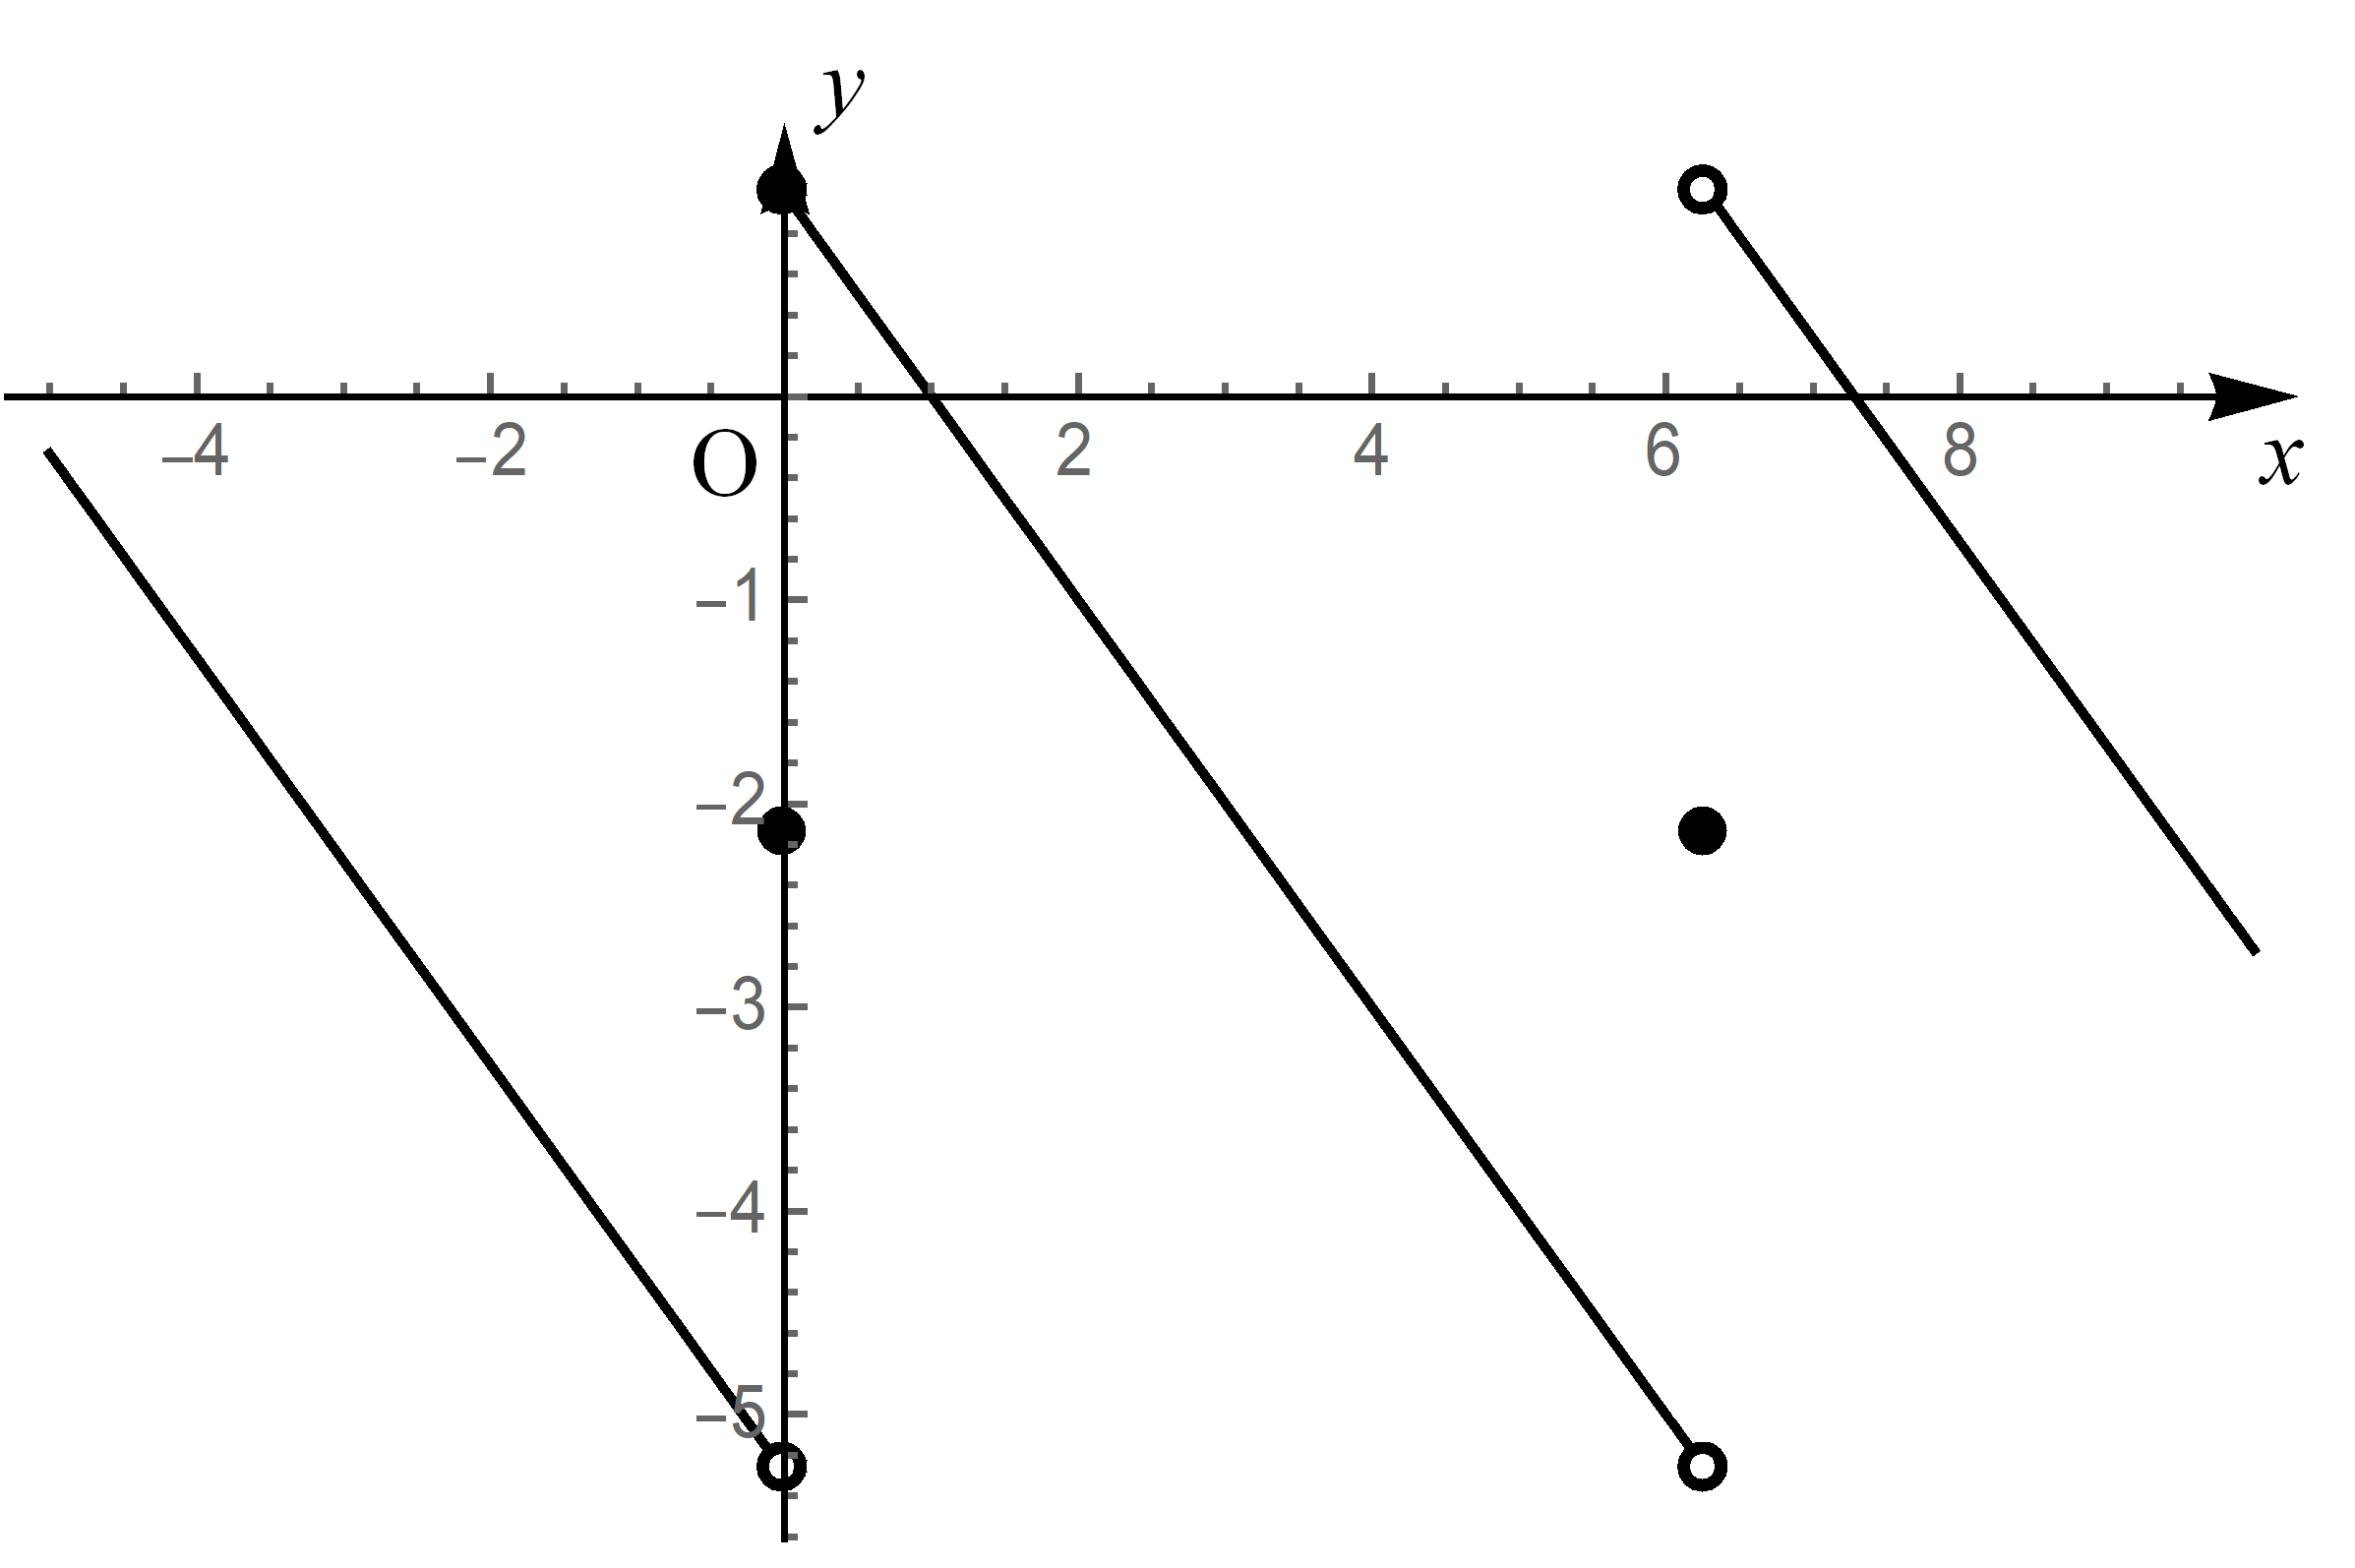
\includegraphics[height=0.3\textheight]{F:/life/2018AutumnTA/Exercises/13/Fig4-1.png}
\end{center}
\caption{习题8.6 4.(1)图示}
\label{4-1}
\end{figure}
(2)$b_n=\frac2\pi\int_0^\pi f(x)\sin nx\mathrm dx=\frac2\pi\int_0^\pi(-x+1)\sin nx\mathrm dx=\frac2{n\pi}\int_0^\pi(x-1)\mathrm d\cos nx\\
=\frac2{n\pi}[(x-1)\cos nx\Big|_0^\pi-\int_0^\pi\cos nx\mathrm dx]=\frac2{n\pi}[(\pi-1)(-1)^n+1-\frac1n\sin nx\Big|_0^\pi]\\
=\frac2{n\pi}[(\pi-1)(-1)^n+1]$

$f(x)\sim\Ser{1}b_n\sin nx=\Ser{1}\frac2{n\pi}[(\pi-1)(-1)^n+1]\sin nx$.

和函数如图~\ref{4-2}所示.
\begin{figure}[H]
\begin{center}
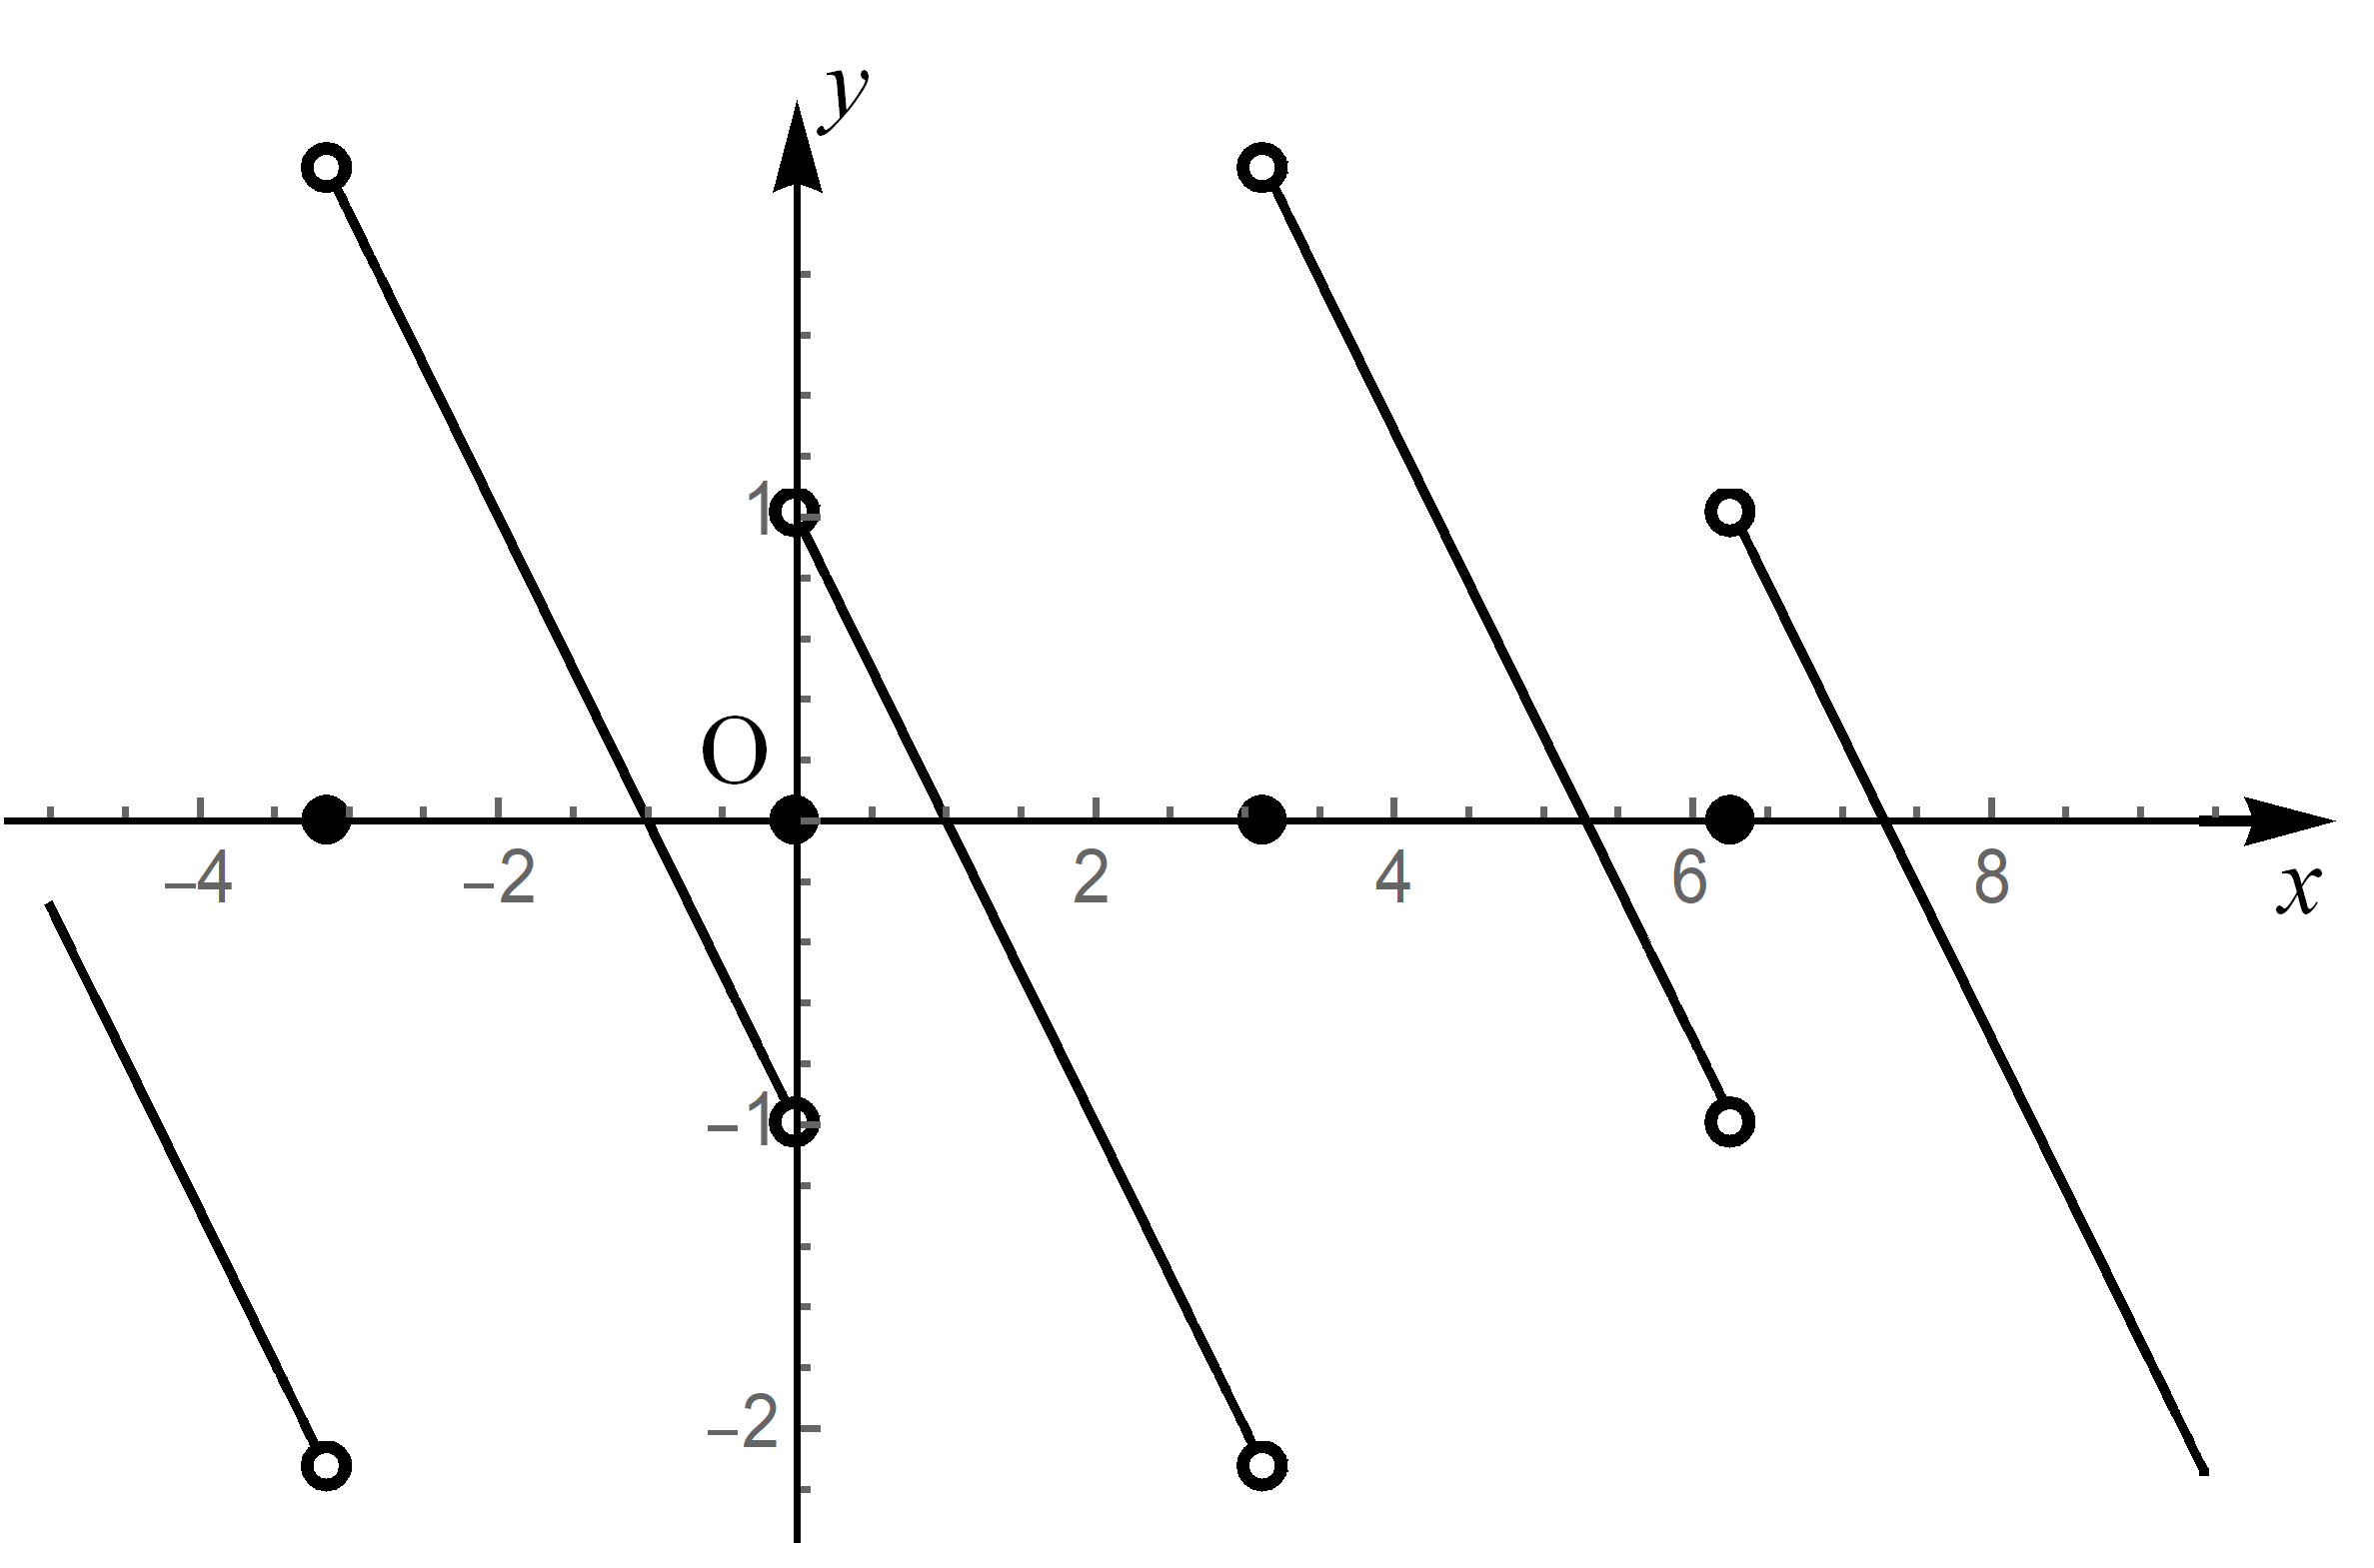
\includegraphics[height=0.3\textheight]{F:/life/2018AutumnTA/Exercises/13/Fig4-2.png}
\end{center}
\caption{习题8.6 4.(2)图示}
\label{4-2}
\end{figure}
(3)$l=\frac\pi2,a_0=\frac2\pi\int_0^\pi f(x)\mathrm dx=\frac2\pi\int_0^\pi(-x+1)\mathrm dx=\frac2\pi(-\frac12x^2+x)\Big|_0^\pi=-\pi+2$

$a_n=\frac2\pi\int_0^\pi f(x)\cos\frac{n\pi}{\frac\pi2}x\mathrm dx=\frac2\pi\int_0^\pi(-x+1)\cos2nx\mathrm dx=\frac2{2n\pi}\int_0^\pi(-x+1)\mathrm d\sin2nx\\
=\frac2{2n\pi}[(-x+1)\sin2nx\Big|_0^\pi+\int_0^\pi\sin2nx\mathrm dx]=\frac1{n\pi}\int_0^\pi\sin2nx\mathrm dx=-\frac1{2n^2\pi}\cos2nx\Big|_0^\pi=0$

$b_n=\frac2\pi\int_0^\pi f(x)\sin2nx\mathrm dx=\frac2\pi\int_0^\pi(-x+1)\sin2nx\mathrm dx=\frac2{2n\pi}\int_0^\pi(x-1)\mathrm d\cos2nx\\
=\frac1{n\pi}[(x-1)\cos2nx\Big|_0^\pi-\int_0^\pi\cos2nx\mathrm dx]=\frac1n$

$f(x)=\frac{a_0}2+\Ser{1}(a_n\cos2nx+b_n\sin2nx)=1-\frac\pi2+\Ser{1}\frac1n\sin2nx$.

和函数如图~\ref{4-3}所示.
\begin{figure}[H]
\begin{center}
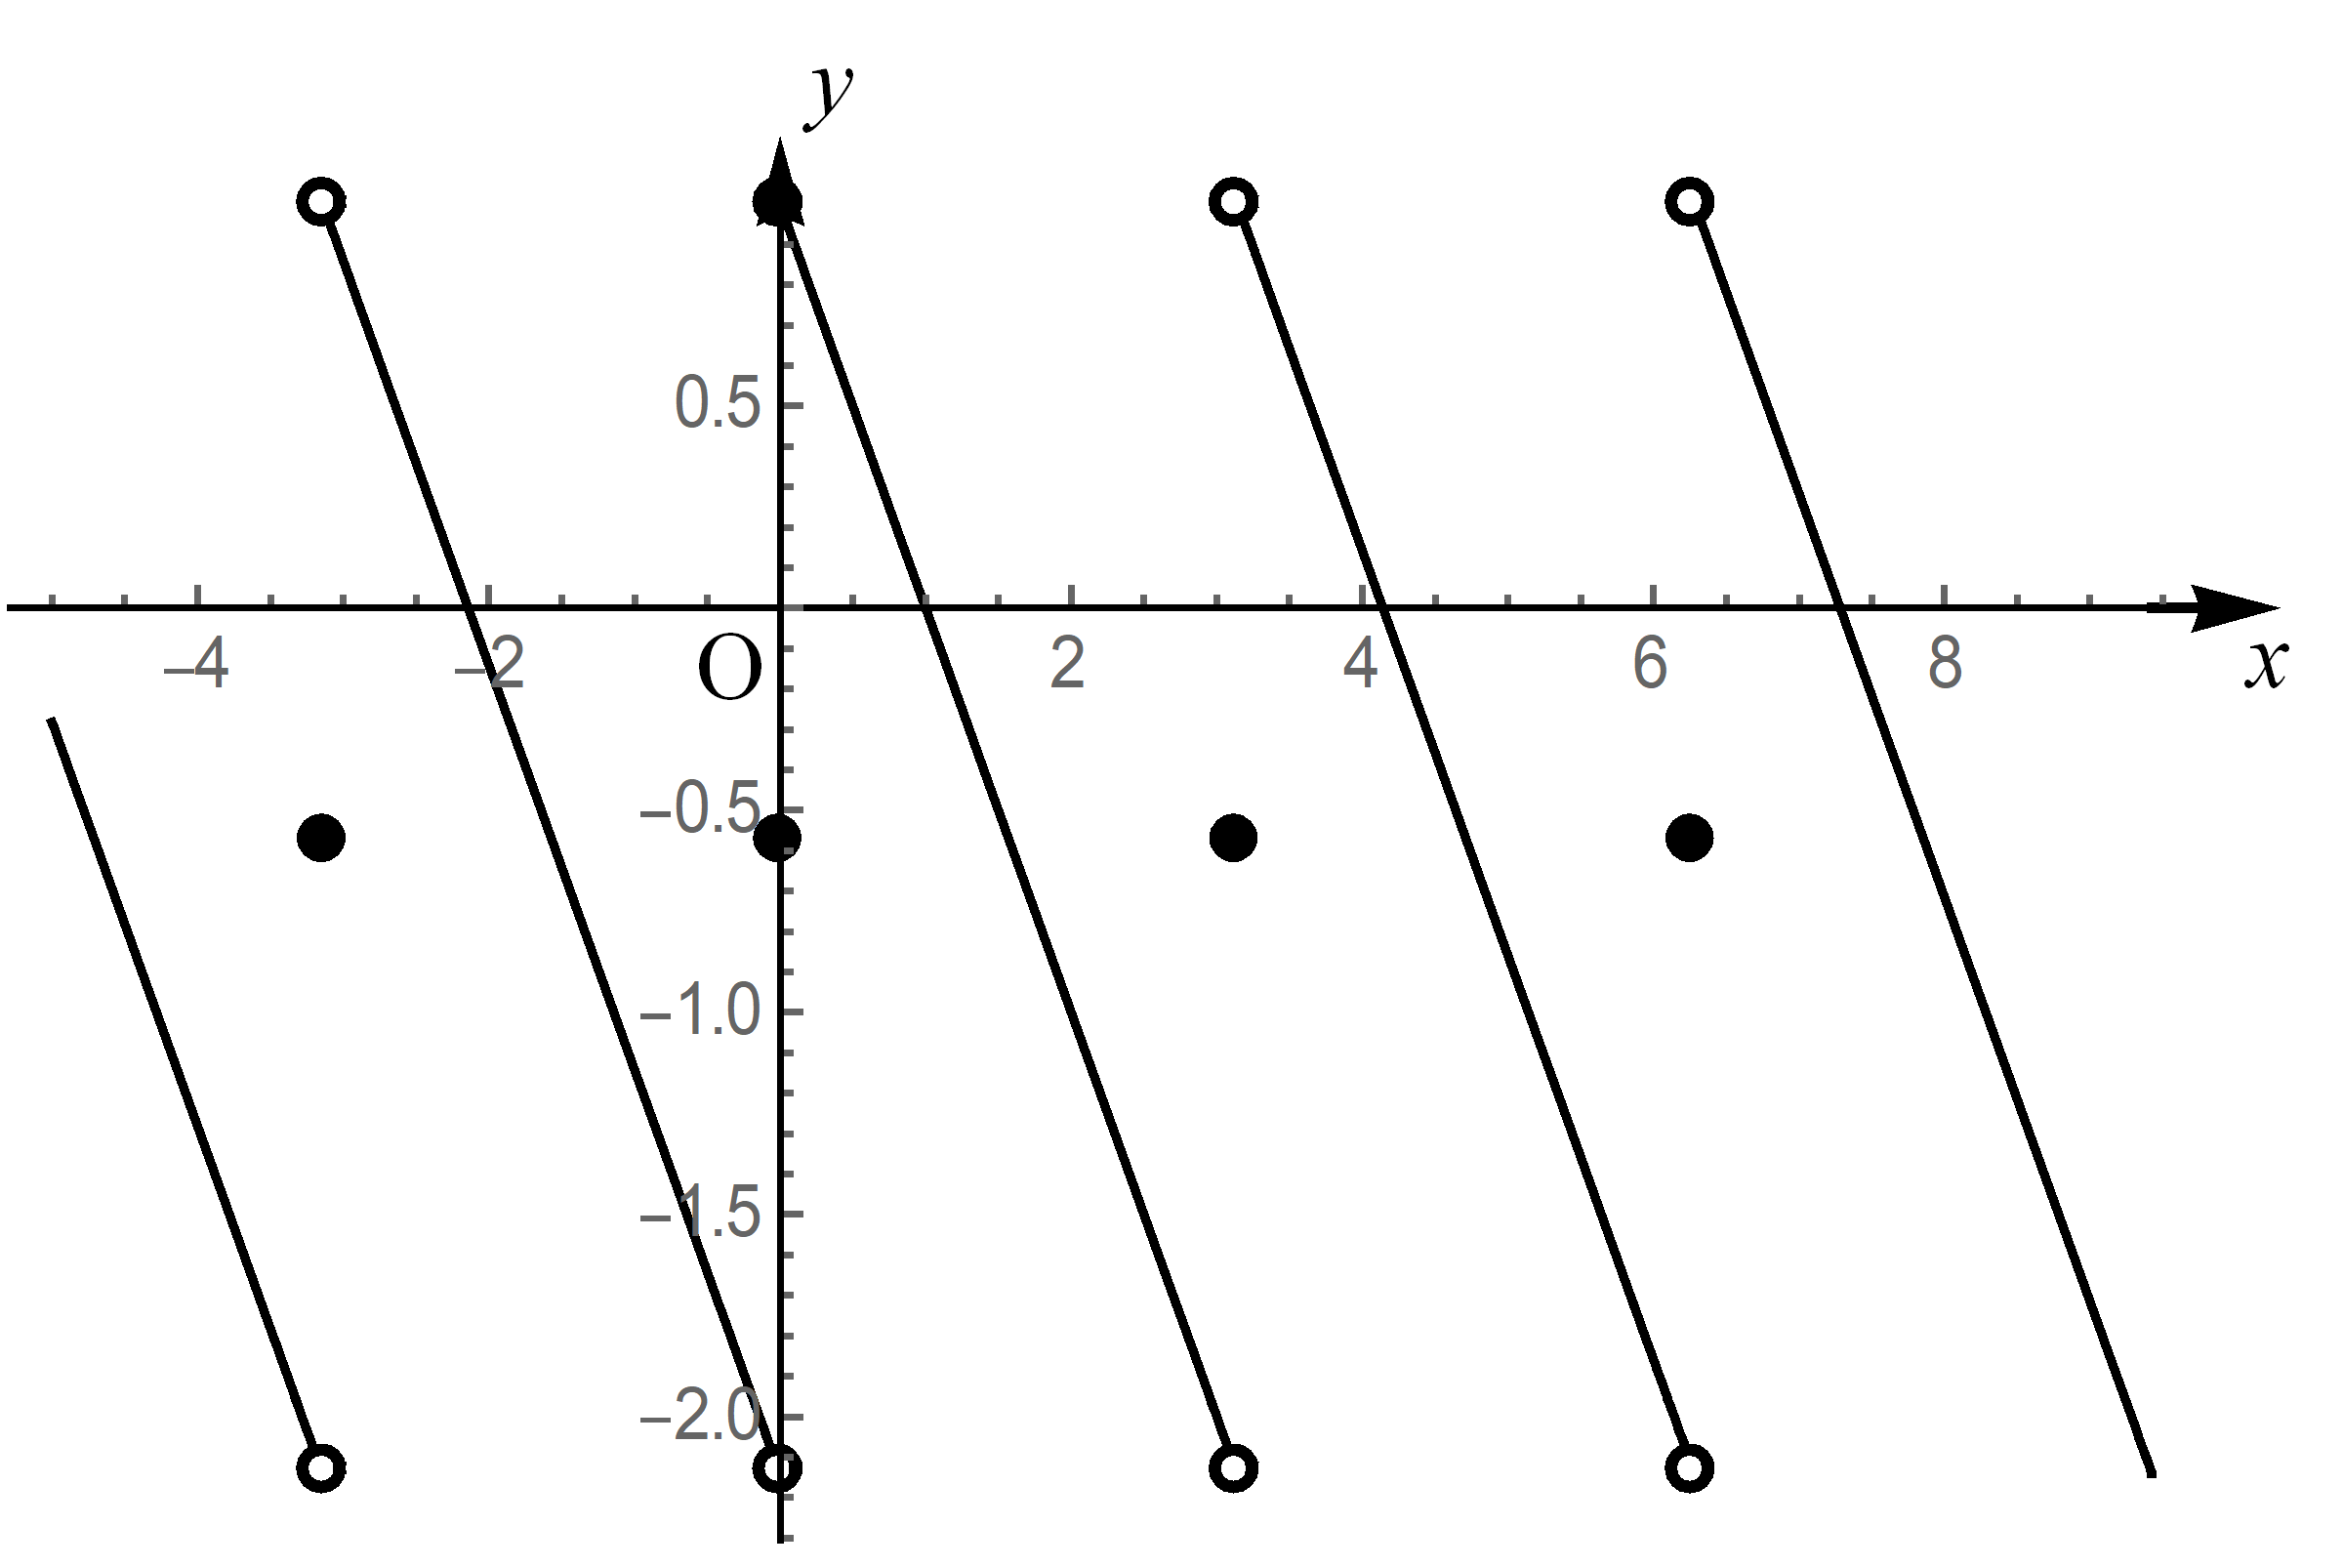
\includegraphics[height=0.3\textheight]{F:/life/2018AutumnTA/Exercises/13/Fig4-3.png}
\end{center}
\caption{习题8.6 4.(3)图示}
\label{4-3}
\end{figure}
(4)$l=1,a_0=\frac11\int_{-1}^1f(x)\mathrm dx=\int_{-1}^1(-x+1)\mathrm dx=2$

$a_n=\frac11\int_{-1}^1f(x)\cos\frac{n\pi}1x\mathrm dx=\int_{-1}^1(-x+1)\cos n\pi x\mathrm dx=\int_{-1}^1\cos n\pi x\mathrm dx=\frac1{n\pi}\sin n\pi x\Big|_{-1}^1\\
=\frac1{n\pi}(\sin n\pi+\sin n\pi)=0$

$b_n=\frac11\int_{-1}^1f(x)\sin\frac{n\pi}1x\mathrm dx=\int_{-1}^1(-x+1)\sin n\pi x\mathrm dx=-\int_{-1}^1x\sin n\pi x\mathrm dx=\frac1{n\pi}\int_{-1}^1x\mathrm d\cos n\pi x\\
=\frac1{n\pi}(x\cos n\pi x\Big|_{-1}^1-\int_{-1}^1\cos n\pi x\mathrm dx)=\frac1{n\pi}(\cos n\pi+\cos n\pi-\frac1{n\pi}\sin n\pi x\Big|_{-1}^1)=\frac{2(-1)^n}{n\pi}$

$f(x)=\frac{a_0}2+\Ser{1}(a_n\cos n\pi x+b_n\sin n\pi x)=1+\Ser{1}\frac{2(-1)^n}{n\pi}\sin n\pi x$.

和函数如图~\ref{4-4}所示.
\begin{figure}[H]
\begin{center}
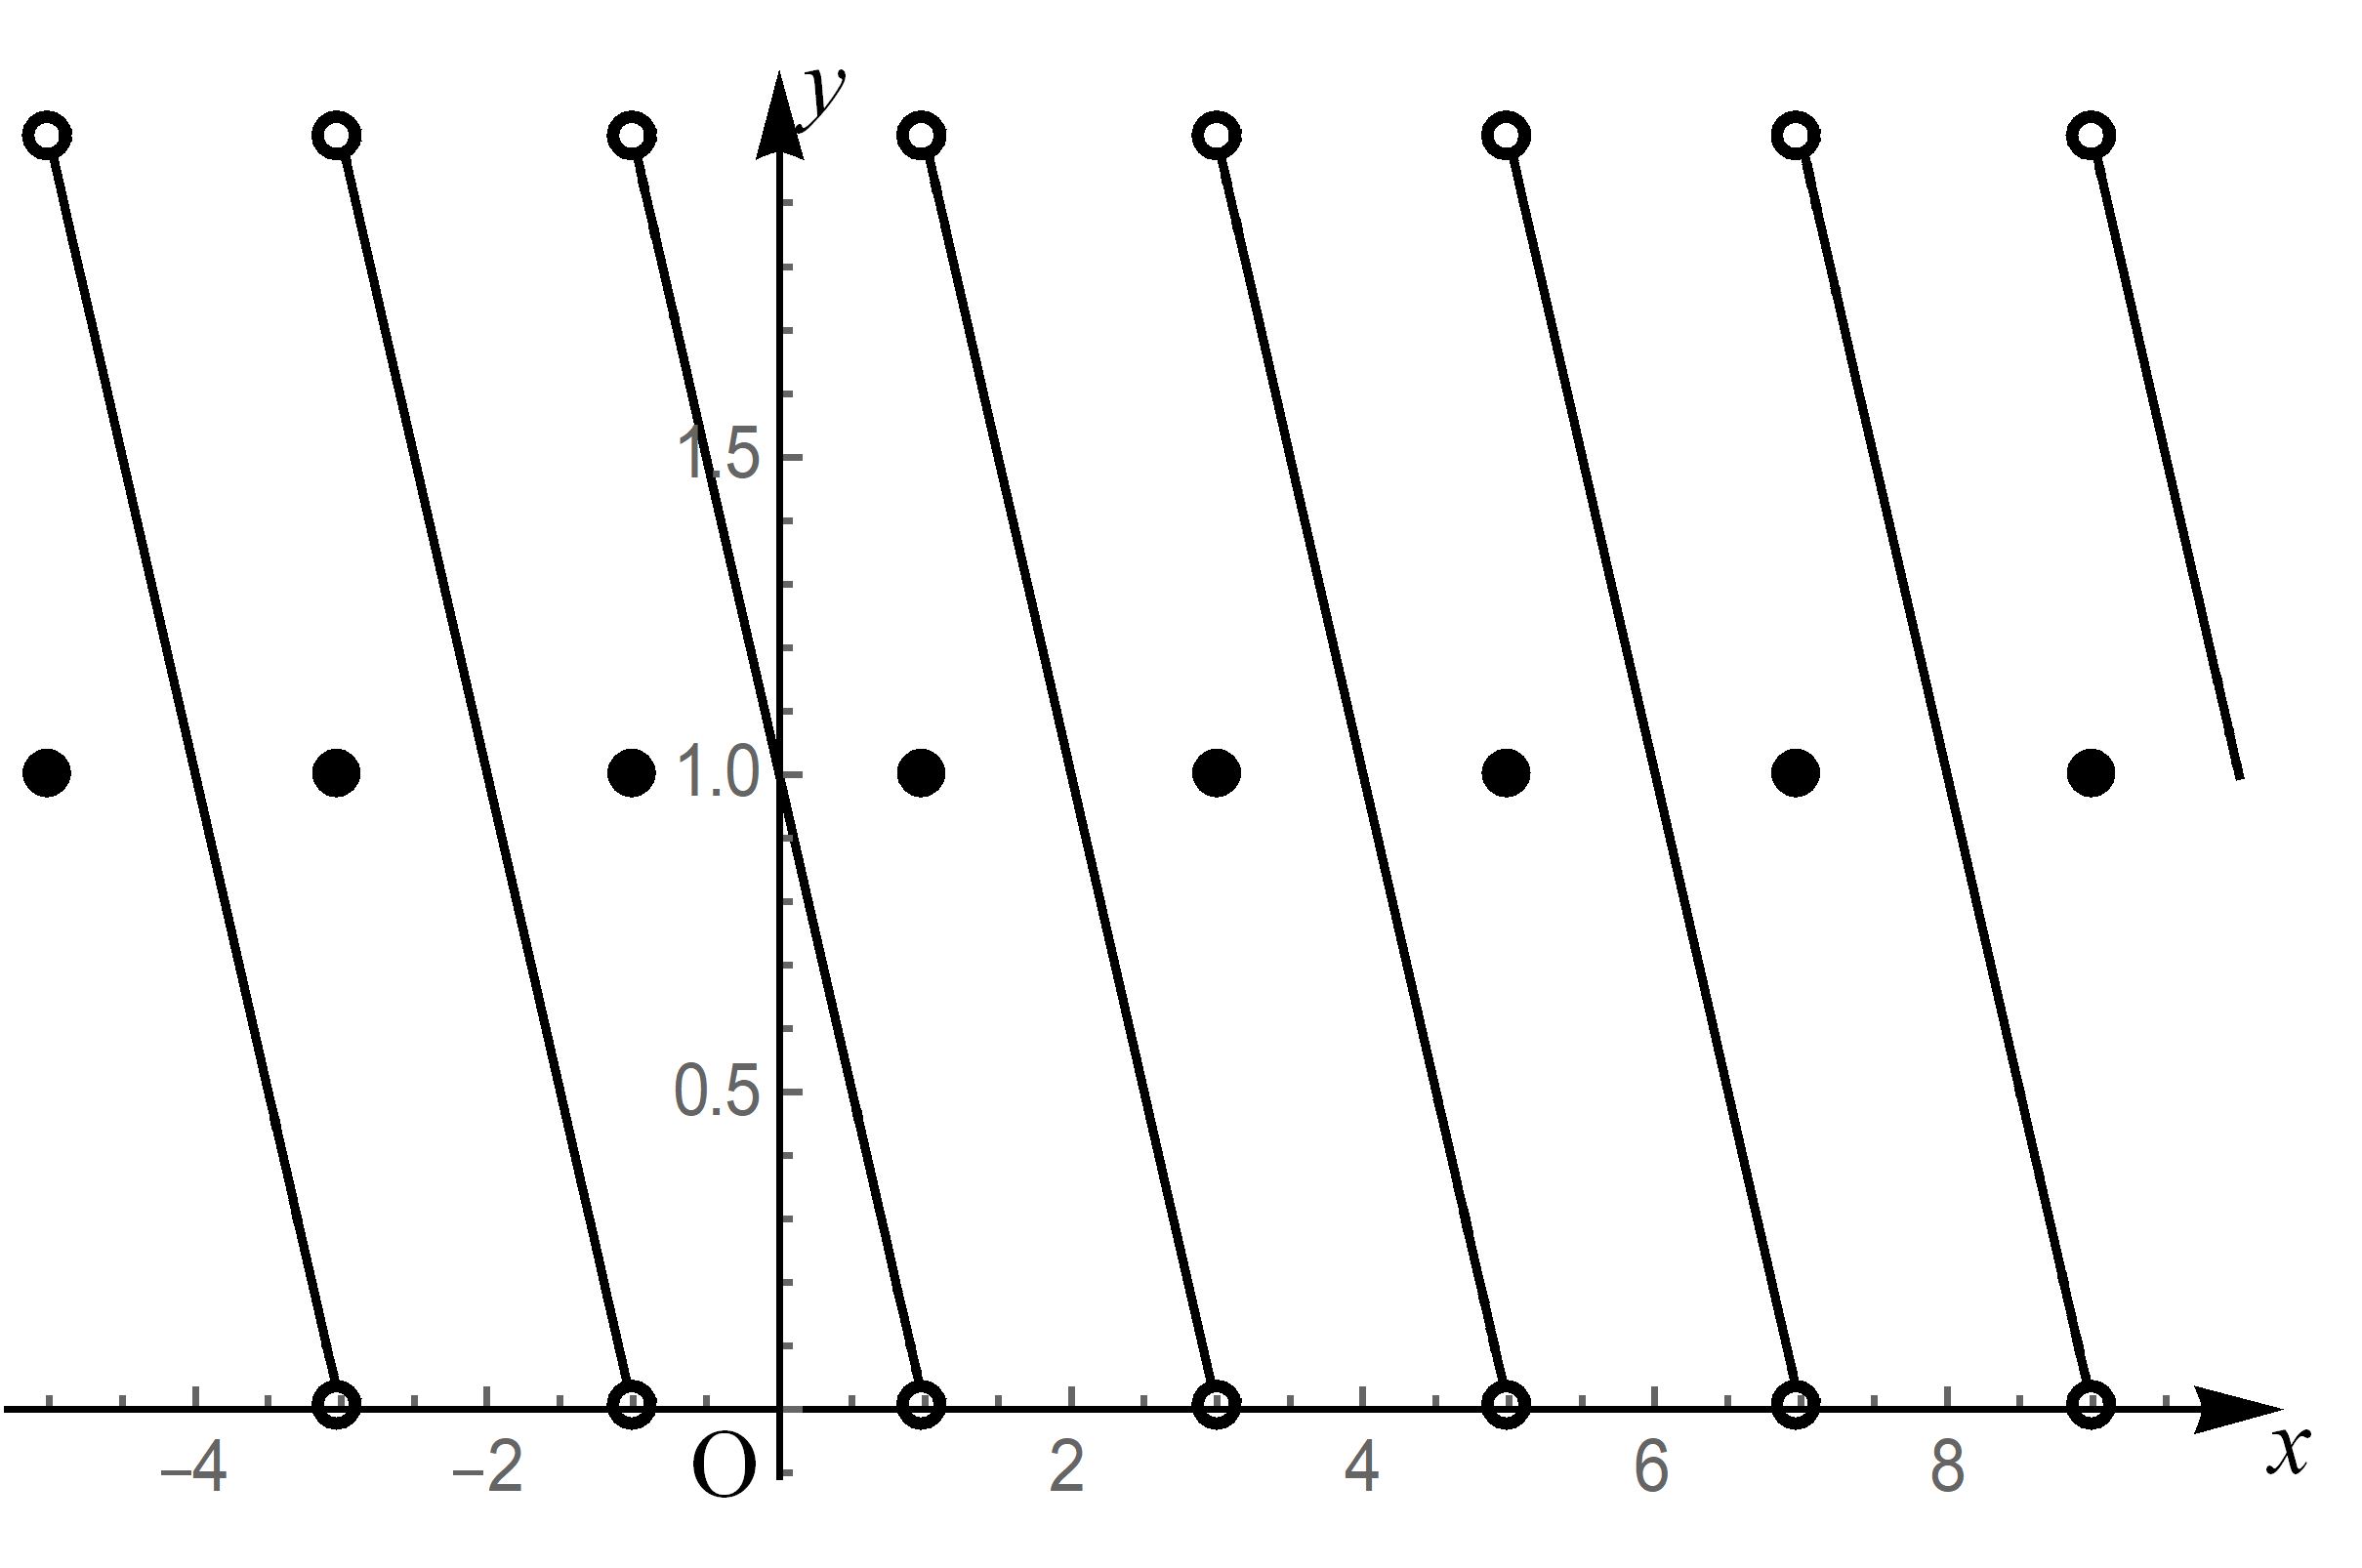
\includegraphics[height=0.3\textheight]{F:/life/2018AutumnTA/Exercises/13/Fig4-4.png}
\end{center}
\caption{习题8.6 4.(4)图示}
\label{4-4}
\end{figure}
\end{enumerate}
\end{document}